Σε αυτή την ενότητα δοκιμάζουμε τον FSMSM με τρόπους τέτοιους ώστε να
αποκαλυφθούν κύρια χαρακτηριστικά και περιορισμοί του.

Αρχικά διενεργούμε μία σειρά πειραμάτων με βάση την πειραματική διάταξη της
ενότητας \ref{subsection:02_04_05:01} για αυξανόμενο μέγιστο ρυθμό
υπερδειγματοληψίας $\mu_{\max} = 2^{\nu_{\max}}$ ώστε να ερευνήσουμε την
απόκριση της μεθόδου \texttt{uf} (και συνεπώς, λόγω της πρακτικά ταυτόσημης
συμπεριφοράς της με τη μέθοδο \texttt{fm}, την απόκριση της \texttt{fm}) σε
ό,τι αφορά τα σφάλματα εκτίμησης προσανατολισμού, και κατά συνέπεια τα σφάλματα
εκτίμησης θέσης, δεδομένων των παρατηρήσεων \ref{remark:loc_prop_or} και
\ref{remark:02_04_02:01}. Για αυτόν τον λόγο διενεργούμε εκατό επαναλήψεις της
μεθόδου πάνω στο σύνολο δεδομένων \texttt{laserazos},\footnote{Το σύνολο
δεδομένων είναι διαθέσιμο στη διεύθυνση
\url{https://censi.science/pub/research/2007-plicp/laserazosSM3.log.gz}
\label{foot:laserazos}} το οποίο διαθέτει $778$ δείγματα πραγματικών
δισδιάστατων σαρώσεων. Η πειραματική διαδικασία που ακολουθήθηκε είναι η ίδια
με αυτήν που περιγράφεται στην ενότητα \ref{subsection:02_04_05:01}---σε
αντίθεση όμως με αυτήν, εδώ έχουμε θέσει $\sigma_R = \sigma_{\bm{M}} = 0.0$ m,
και ο μέγιστος ρυθμός δειγματοληψίας κυμαίνεται από $\mu_{\max} = 2^0$ έως
$\mu_{\max} = 2^6$. Κατά συνέπεια για να προκύψει το σχήμα
\ref{fig:02_04_06:01} διενεργήθηκαν $100 \times 778 \times |\{0,1,\dots,6\}|
\simeq 5.4\cdot 10^5$ ευθυγραμμίσεις πραγματικών με εικονικές σαρώσεις. Το
σχήμα αυτό απεικονίζει το μέσο όρο σφάλματος εκτίμησης ανά επανάληψη εκτέλεσης
πάνω στο σύνολο δεδομένων και την τυπική απόκλιση γύρω από αυτόν, για τα
σφάλματα εκτίμησης προσανατολισμού και θέσης (άνω και μεσαία σειρά), και το
μέσο χρόνο εκτέλεσης ανά ευθυγράμμιση (κάτω σειρά).

\begin{figure}\centering
  \definecolor{r}{rgb}{1 0 0}
% GNUPLOT: LaTeX picture with Postscript
\begingroup
  \makeatletter
  \providecommand\color[2][]{%
    \GenericError{(gnuplot) \space\space\space\@spaces}{%
      Package color not loaded in conjunction with
      terminal option `colourtext'%
    }{See the gnuplot documentation for explanation.%
    }{Either use 'blacktext' in gnuplot or load the package
      color.sty in LaTeX.}%
    \renewcommand\color[2][]{}%
  }%
  \providecommand\includegraphics[2][]{%
    \GenericError{(gnuplot) \space\space\space\@spaces}{%
      Package graphicx or graphics not loaded%
    }{See the gnuplot documentation for explanation.%
    }{The gnuplot epslatex terminal needs graphicx.sty or graphics.sty.}%
    \renewcommand\includegraphics[2][]{}%
  }%
  \providecommand\rotatebox[2]{#2}%
  \@ifundefined{ifGPcolor}{%
    \newif\ifGPcolor
    \GPcolorfalse
  }{}%
  \@ifundefined{ifGPblacktext}{%
    \newif\ifGPblacktext
    \GPblacktexttrue
  }{}%
  % define a \g@addto@macro without @ in the name:
  \let\gplgaddtomacro\g@addto@macro
  % define empty templates for all commands taking text:
  \gdef\gplfronttext{}%
  \gdef\gplfronttext{}%
  \makeatother
  \ifGPblacktext
    % no textcolor at all
    \def\colorrgb#1{}%
    \def\colorgray#1{}%
  \else
    % gray or color?
    \ifGPcolor
      \def\colorrgb#1{\color[rgb]{#1}}%
      \def\colorgray#1{\color[gray]{#1}}%
      \expandafter\def\csname LTw\endcsname{\color{white}}%
      \expandafter\def\csname LTb\endcsname{\color{black}}%
      \expandafter\def\csname LTa\endcsname{\color{black}}%
      \expandafter\def\csname LT0\endcsname{\color[rgb]{1,0,0}}%
      \expandafter\def\csname LT1\endcsname{\color[rgb]{0,1,0}}%
      \expandafter\def\csname LT2\endcsname{\color[rgb]{0,0,1}}%
      \expandafter\def\csname LT3\endcsname{\color[rgb]{1,0,1}}%
      \expandafter\def\csname LT4\endcsname{\color[rgb]{0,1,1}}%
      \expandafter\def\csname LT5\endcsname{\color[rgb]{1,1,0}}%
      \expandafter\def\csname LT6\endcsname{\color[rgb]{0,0,0}}%
      \expandafter\def\csname LT7\endcsname{\color[rgb]{1,0.3,0}}%
      \expandafter\def\csname LT8\endcsname{\color[rgb]{0.5,0.5,0.5}}%
    \else
      % gray
      \def\colorrgb#1{\color{black}}%
      \def\colorgray#1{\color[gray]{#1}}%
      \expandafter\def\csname LTw\endcsname{\color{white}}%
      \expandafter\def\csname LTb\endcsname{\color{black}}%
      \expandafter\def\csname LTa\endcsname{\color{black}}%
      \expandafter\def\csname LT0\endcsname{\color{black}}%
      \expandafter\def\csname LT1\endcsname{\color{black}}%
      \expandafter\def\csname LT2\endcsname{\color{black}}%
      \expandafter\def\csname LT3\endcsname{\color{black}}%
      \expandafter\def\csname LT4\endcsname{\color{black}}%
      \expandafter\def\csname LT5\endcsname{\color{black}}%
      \expandafter\def\csname LT6\endcsname{\color{black}}%
      \expandafter\def\csname LT7\endcsname{\color{black}}%
      \expandafter\def\csname LT8\endcsname{\color{black}}%
    \fi
  \fi
    \setlength{\unitlength}{0.0500bp}%
    \ifx\gptboxheight\undefined%
      \newlength{\gptboxheight}%
      \newlength{\gptboxwidth}%
      \newsavebox{\gptboxtext}%
    \fi%
    \setlength{\fboxrule}{0.5pt}%
    \setlength{\fboxsep}{1pt}%
\begin{picture}(5000.00,8000.00)%
    \gplgaddtomacro\gplfronttext{%
      \colorrgb{0.15,0.15,0.15}%
      \put(518,5795){\makebox(0,0)[r]{\strut{}$10$\texttt{e}$-$$4$}}%
      \colorrgb{0.15,0.15,0.15}%
      \put(518,6330){\makebox(0,0)[r]{\strut{}$10$\texttt{e}$-$$3$}}%
      \colorrgb{0.15,0.15,0.15}%
      \put(518,6864){\makebox(0,0)[r]{\strut{}$10$\texttt{e}$-$$2$}}%
      \colorrgb{0.15,0.15,0.15}%
      \put(518,7399){\makebox(0,0)[r]{\strut{}$10$\texttt{e}$-$$1$}}%
    }%
    \gplgaddtomacro\gplfronttext{%
      \colorrgb{0.00,0.00,0.00}%
      \put(2587,7619){\makebox(0,0){\strut{}Σφάλμα εκτίμησης προσανατολισμού συναρτήσει $\mu_{\max}$ [rad]}}%
    }%
    \gplgaddtomacro\gplfronttext{%
      \colorrgb{1.00,0.00,0.00}%
      \put(4656,5874){\makebox(0,0)[l]{\strut{}\color{r}{\scriptsize $0.65$}}}%
      \colorrgb{1.00,0.00,0.00}%
      \put(4656,6024){\makebox(0,0)[l]{\strut{}\color{r}{\scriptsize $0.68$}}}%
      \colorrgb{1.00,0.00,0.00}%
      \put(4656,6163){\makebox(0,0)[l]{\strut{}\color{r}{\scriptsize $0.54$}}}%
      \colorrgb{1.00,0.00,0.00}%
      \put(4656,6302){\makebox(0,0)[l]{\strut{}\color{r}{\scriptsize $0.29$}}}%
      \colorrgb{1.00,0.00,0.00}%
      \put(4656,6582){\makebox(0,0)[l]{\strut{}\color{r}{\scriptsize $0.22$}}}%
      \colorrgb{1.00,0.00,0.00}%
      \put(4656,6931){\makebox(0,0)[l]{\strut{}\color{r}{\scriptsize $0.54$}}}%
      \colorrgb{1.00,0.00,0.00}%
      \put(4656,7072){\makebox(0,0)[l]{\strut{}\color{r}{\scriptsize ΑΠ}}}%
    }%
    \gplgaddtomacro\gplfronttext{%
    }%
    \gplgaddtomacro\gplfronttext{%
      \colorrgb{0.15,0.15,0.15}%
      \put(518,3337){\makebox(0,0)[r]{\strut{}$10$\texttt{e}$-$$4$}}%
      \colorrgb{0.15,0.15,0.15}%
      \put(518,3738){\makebox(0,0)[r]{\strut{}$10$\texttt{e}$-$$3$}}%
      \colorrgb{0.15,0.15,0.15}%
      \put(518,4139){\makebox(0,0)[r]{\strut{}$10$\texttt{e}$-$$2$}}%
      \colorrgb{0.15,0.15,0.15}%
      \put(518,4540){\makebox(0,0)[r]{\strut{}$10$\texttt{e}$-$$1$}}%
      \colorrgb{0.15,0.15,0.15}%
      \put(518,4941){\makebox(0,0)[r]{\strut{}$10$\texttt{e}$+$$0$}}%
    }%
    \gplgaddtomacro\gplfronttext{%
      \colorrgb{0.00,0.00,0.00}%
      \put(2587,5161){\makebox(0,0){\strut{}Σφάλμα εκτίμησης θέσης συναρτήσει $\mu_{\max}$ [m]}}%
    }%
    \gplgaddtomacro\gplfronttext{%
      \colorrgb{1.00,0.00,0.00}%
      \put(4656,3462){\makebox(0,0)[l]{\strut{}\color{r}{\scriptsize $0.62$}}}%
      \colorrgb{1.00,0.00,0.00}%
      \put(4656,3596){\makebox(0,0)[l]{\strut{}\color{r}{\scriptsize $0.58$}}}%
      \colorrgb{1.00,0.00,0.00}%
      \put(4656,3738){\makebox(0,0)[l]{\strut{}\color{r}{\scriptsize $0.30$}}}%
      \colorrgb{1.00,0.00,0.00}%
      \put(4656,3947){\makebox(0,0)[l]{\strut{}\color{r}{\scriptsize $0.23$}}}%
      \colorrgb{1.00,0.00,0.00}%
      \put(4656,4200){\makebox(0,0)[l]{\strut{}\color{r}{\scriptsize $0.23$}}}%
      \colorrgb{1.00,0.00,0.00}%
      \put(4656,4454){\makebox(0,0)[l]{\strut{}\color{r}{\scriptsize $0.39$}}}%
      \colorrgb{1.00,0.00,0.00}%
      \put(4656,4616){\makebox(0,0)[l]{\strut{}\color{r}{\scriptsize ΑΠ}}}%
    }%
    \gplgaddtomacro\gplfronttext{%
    }%
    \gplgaddtomacro\gplfronttext{%
      \colorrgb{0.15,0.15,0.15}%
      \put(518,880){\makebox(0,0)[r]{\strut{}$0$}}%
      \colorrgb{0.15,0.15,0.15}%
      \put(518,1081){\makebox(0,0)[r]{\strut{}$20$}}%
      \colorrgb{0.15,0.15,0.15}%
      \put(518,1281){\makebox(0,0)[r]{\strut{}$40$}}%
      \colorrgb{0.15,0.15,0.15}%
      \put(518,1482){\makebox(0,0)[r]{\strut{}$60$}}%
      \colorrgb{0.15,0.15,0.15}%
      \put(518,1682){\makebox(0,0)[r]{\strut{}$80$}}%
      \colorrgb{0.15,0.15,0.15}%
      \put(518,1883){\makebox(0,0)[r]{\strut{}$100$}}%
      \colorrgb{0.15,0.15,0.15}%
      \put(518,2083){\makebox(0,0)[r]{\strut{}$120$}}%
      \colorrgb{0.15,0.15,0.15}%
      \put(518,2284){\makebox(0,0)[r]{\strut{}$140$}}%
      \colorrgb{0.15,0.15,0.15}%
      \put(518,2484){\makebox(0,0)[r]{\strut{}$160$}}%
      \colorrgb{0.15,0.15,0.15}%
      \put(771,660){\makebox(0,0){\strut{}$2^0$}}%
      \colorrgb{0.15,0.15,0.15}%
      \put(1376,660){\makebox(0,0){\strut{}$2^1$}}%
      \colorrgb{0.15,0.15,0.15}%
      \put(1982,660){\makebox(0,0){\strut{}$2^2$}}%
      \colorrgb{0.15,0.15,0.15}%
      \put(2587,660){\makebox(0,0){\strut{}$2^3$}}%
      \colorrgb{0.15,0.15,0.15}%
      \put(3192,660){\makebox(0,0){\strut{}$2^4$}}%
      \colorrgb{0.15,0.15,0.15}%
      \put(3798,660){\makebox(0,0){\strut{}$2^5$}}%
      \colorrgb{0.15,0.15,0.15}%
      \put(4403,660){\makebox(0,0){\strut{}$2^6$}}%
    }%
    \gplgaddtomacro\gplfronttext{%
      \colorrgb{0.00,0.00,0.00}%
      \put(2587,2704){\makebox(0,0){\strut{}Ολικός χρόνος εκτέλεσης συναρτήσει $\mu_{\max}$ [ms]}}%
    }%
    \gplgaddtomacro\gplfronttext{%
      \colorrgb{1.00,0.00,0.00}%
      \put(4656,898){\makebox(0,0)[l]{\strut{}\color{r}{\scriptsize ΑΠ}}}%
      \colorrgb{1.00,0.00,0.00}%
      \put(4656,1025){\makebox(0,0)[l]{\strut{}\color{r}{\scriptsize $2.14$}}}%
      \colorrgb{1.00,0.00,0.00}%
      \put(4656,1171){\makebox(0,0)[l]{\strut{}\color{r}{\scriptsize $1.99$}}}%
      \colorrgb{1.00,0.00,0.00}%
      \put(4656,1381){\makebox(0,0)[l]{\strut{}\color{r}{\scriptsize $1.72$}}}%
      \colorrgb{1.00,0.00,0.00}%
      \put(4656,1633){\makebox(0,0)[l]{\strut{}\color{r}{\scriptsize $1.50$}}}%
      \colorrgb{1.00,0.00,0.00}%
      \put(4656,1793){\makebox(0,0)[l]{\strut{}\color{r}{\scriptsize $1.21$}}}%
      \colorrgb{1.00,0.00,0.00}%
      \put(4656,2096){\makebox(0,0)[l]{\strut{}\color{r}{\scriptsize $1.33$}}}%
    }%
    \gplgaddtomacro\gplfronttext{%
    }%
    \put(0,0){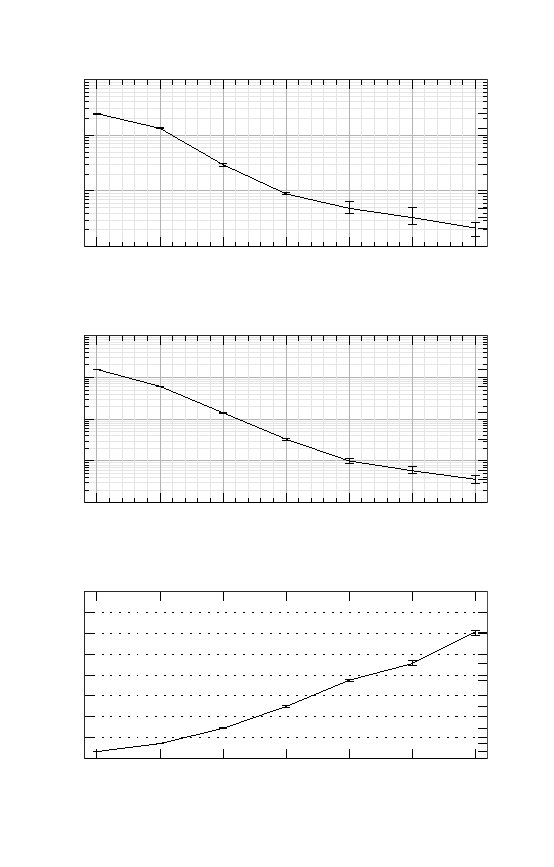
\includegraphics{./figures/parts/02/chapters/04/sections/06/errorbar_varying_resolution}}%
    \gplfronttext
  \end{picture}%
\endgroup


  \caption{\small Κύρια στατιστικά της μεθόδου \texttt{uf} σε εκατό επαναλήψεις
           πάνω στο σύνολο δεδομένων \texttt{laserazos}. Στον δεξιό κάθετο άξονα
           σημειώνονται οι τιμές των κλασμάτων μετρικών διαδοχικών ρυθμών
           υπερδειγματοληψίας---π.χ.
           $\dfrac{e_{\theta}|_{\mu_{\max} = 2^1}}{e_{\theta}|_{\mu_{\max} = 2^0}} = 0.54$,
           $\dfrac{e_{xy}|_{\mu_{\max} = 2^1}}{e_{xy}|_{\mu_{\max} = 2^0}} = 0.39$,
           και $\dfrac{T|_{\mu_{\max} = 2^1}}{T|_{\mu_{\max} = 2^0}} = 2.14$. Η
           συντομογραφία ΑΠ σημαίνει την απροσδιοριστία}
  \label{fig:02_04_06:01}
\end{figure}

Σε αυτά τα διαγράμματα παρατηρούμε πως ο διπλασιασμός του ρυθμού
υπερδειγματοληψίας επιφέρει μεταβλητή μείωση των σφαλμάτων και μεταβλητή αύξηση
του χρόνου εκτέλεσης, πάντα όμως γύρω από τον παράγοντα δύο. Τα άνω δύο
διαγράμματα επιβεβαιώνουν την παρατήρηση \ref{remark:loc_prop_or}, δηλαδή πως
χαμηλότερα σφάλματα εκτίμησης προσανατολισμού οδηγούν σε χαμηλότερα σφάλματα
εκτίμησης θέσης, και την παρατήρηση \ref{remark:02_04_02:01}, δηλαδή το
αντίστροφο. Ταυτόχρονα παρατηρείται πως, εν γένει, η αύξηση του ρυθμού
υπερδειγματοληψίας οδηγεί σε επιβράδυνση της αύξησης του μέσου σφάλματος και
του χρόνου εκτέλεσης: όσο αυξάνει ο ρυθμός υπερδειγματοληψίας τόσο  αυξάνει το
κλάσμα ανάμεσα σε διαδοχικές τιμές των μετρικών μέσου σφάλματος και χρόνου
εκτέλεσης.


Στο σχήμα \ref{fig:02_04_06:02} παρατίθεται ένα τυπικό παράδειγμα εξέλιξης της
ευθυγράμμισης μίας πραγματικής δισδιάστατης πανοραμικής σάρωσης με εικονικές
σαρώσεις μέσω της μεθόδου FSMSM, και συγκεκριμένα μέσω της μεθόδου \texttt{x1}.
Εδώ η πραγματική σάρωση επιβαρύνεται με διαταραχές τυπικής απόκλισης $\sigma_R
= 0.05$ m, και οι εικονικές σαρώσεις προκύπτουν απο χάρτη ο οποίος αναπαριστά
στην εντέλεια το περιβάλλον του αισθητήρα lidar ($\sigma_{\bm{M}} = 0.0$ m). Η
άνω σειρά του σχήματος παρουσιάζει την αρχική συνθήκη ευθυγράμμισης στο χάρτη
που σημειώνεται με μαύρο περίγραμμα στα αριστερά, δηλαδή την πραγματική στάση
του αισθητήρα (μαύρο χρώμα) και την αρχική εκτιμώμενή του στάση (ματζέντα). Η
πραγματική στάση του αισθητήρα είναι $\bm{p} = [0.563, 2.1, 0.47]^\top$ και η
αρχική εκτίμησή της $\hat{\bm{p}} = [0.26, 2.35, 1.738]^\top$. Στα δεξιά
παρουσιάζεται η πραγματική σάρωση με μαύρο χρώμα, και η εικονική σάρωση που
υπολογίζεται από την αρχική εκτίμηση της στάσης του αισθητήρα με ματζέντα, στο
τοπικό σύστημα συντεταγμένων της κάθε μίας. Στην πρώτη στήλη του
περιγεγραμμένου διαγράμματος παρουσιάζονται το πραγματικό διάνυσμα μετρήσεων
(μαύρο) και το εικονικό διάνυσμα μετρήσεων αμέσως μετά την εφαρμογή του βήματος
εκτίμησης του προσανατολισμού της πραγματικής στάσης του αισθητήρα (με
ματζέντα---Αλγόριθμος \ref{alg:02_04_04:rc}). Στη δεύτερη στήλη παρουσιάζονται
η πραγματική στάση του αισθητήρα και οι αντιστοιχούσες εκτιμήσεις της FSMSM για
αυτή. Στην τρίτη στήλη παρουσιάζονται τα διαγράμματα εξέλιξης του ολικού
σφάλματος εκτίμησης (με μπλε χρώμα) και της τιμής της μετρικής CAER (κόκκινο).
Οι υπόλοιπες στήλες παρουσιάζουν τα ίδια περιεχόμενα αμέσως μετά την εφαρμογή
του βήματος εκτίμησης της θέσης της πραγματικής στάσης του αισθητήρα
(Αλγόριθμος \ref{alg:icte}).  Η τελευταία σειρά του σχήματος παρουσιάζει το
αποτέλεσμα του FSMSM στον Ευκλείδειο χώρο (αριστερά)---δηλαδή την τελική
εκτίμηση της στάσης του αισθητήρα---και στο χώρο μετρήσεων---δηλαδή την
ευθυγράμμιση της εικονικής σάρωσης από την τελική εκτίμηση στάσης με την
πραγματική σάρωση. Η τελική εκτίμηση της FSMSM είναι $\hat{\bm{p}} = [0.55854,
2.09692, 0.46509]^\top$, με σφάλμα εκτίμησης θέσης $e_{xy} = 0.00542$ m και
σφάλμα εκτίμησης προσανατολισμού $e_{\theta} = 0.00491$ rad.

\begin{figure}
  \begin{subfigure}{\linewidth}\hspace{-0.25cm}
    % GNUPLOT: LaTeX picture with Postscript
\begingroup
  \makeatletter
  \providecommand\color[2][]{%
    \GenericError{(gnuplot) \space\space\space\@spaces}{%
      Package color not loaded in conjunction with
      terminal option `colourtext'%
    }{See the gnuplot documentation for explanation.%
    }{Either use 'blacktext' in gnuplot or load the package
      color.sty in LaTeX.}%
    \renewcommand\color[2][]{}%
  }%
  \providecommand\includegraphics[2][]{%
    \GenericError{(gnuplot) \space\space\space\@spaces}{%
      Package graphicx or graphics not loaded%
    }{See the gnuplot documentation for explanation.%
    }{The gnuplot epslatex terminal needs graphicx.sty or graphics.sty.}%
    \renewcommand\includegraphics[2][]{}%
  }%
  \providecommand\rotatebox[2]{#2}%
  \@ifundefined{ifGPcolor}{%
    \newif\ifGPcolor
    \GPcolorfalse
  }{}%
  \@ifundefined{ifGPblacktext}{%
    \newif\ifGPblacktext
    \GPblacktexttrue
  }{}%
  % define a \g@addto@macro without @ in the name:
  \let\gplgaddtomacro\g@addto@macro
  % define empty templates for all commands taking text:
  \gdef\gplfronttext{}%
  \gdef\gplfronttext{}%
  \makeatother
  \ifGPblacktext
    % no textcolor at all
    \def\colorrgb#1{}%
    \def\colorgray#1{}%
  \else
    % gray or color?
    \ifGPcolor
      \def\colorrgb#1{\color[rgb]{#1}}%
      \def\colorgray#1{\color[gray]{#1}}%
      \expandafter\def\csname LTw\endcsname{\color{white}}%
      \expandafter\def\csname LTb\endcsname{\color{black}}%
      \expandafter\def\csname LTa\endcsname{\color{black}}%
      \expandafter\def\csname LT0\endcsname{\color[rgb]{1,0,0}}%
      \expandafter\def\csname LT1\endcsname{\color[rgb]{0,1,0}}%
      \expandafter\def\csname LT2\endcsname{\color[rgb]{0,0,1}}%
      \expandafter\def\csname LT3\endcsname{\color[rgb]{1,0,1}}%
      \expandafter\def\csname LT4\endcsname{\color[rgb]{0,1,1}}%
      \expandafter\def\csname LT5\endcsname{\color[rgb]{1,1,0}}%
      \expandafter\def\csname LT6\endcsname{\color[rgb]{0,0,0}}%
      \expandafter\def\csname LT7\endcsname{\color[rgb]{1,0.3,0}}%
      \expandafter\def\csname LT8\endcsname{\color[rgb]{0.5,0.5,0.5}}%
    \else
      % gray
      \def\colorrgb#1{\color{black}}%
      \def\colorgray#1{\color[gray]{#1}}%
      \expandafter\def\csname LTw\endcsname{\color{white}}%
      \expandafter\def\csname LTb\endcsname{\color{black}}%
      \expandafter\def\csname LTa\endcsname{\color{black}}%
      \expandafter\def\csname LT0\endcsname{\color{black}}%
      \expandafter\def\csname LT1\endcsname{\color{black}}%
      \expandafter\def\csname LT2\endcsname{\color{black}}%
      \expandafter\def\csname LT3\endcsname{\color{black}}%
      \expandafter\def\csname LT4\endcsname{\color{black}}%
      \expandafter\def\csname LT5\endcsname{\color{black}}%
      \expandafter\def\csname LT6\endcsname{\color{black}}%
      \expandafter\def\csname LT7\endcsname{\color{black}}%
      \expandafter\def\csname LT8\endcsname{\color{black}}%
    \fi
  \fi
    \setlength{\unitlength}{0.0500bp}%
    \ifx\gptboxheight\undefined%
      \newlength{\gptboxheight}%
      \newlength{\gptboxwidth}%
      \newsavebox{\gptboxtext}%
    \fi%
    \setlength{\fboxrule}{0.5pt}%
    \setlength{\fboxsep}{1pt}%
\begin{picture}(8000.00,2600.00)%
    \gplgaddtomacro\gplfronttext{%
      \colorrgb{0.15,0.15,0.15}%
      \put(1425,260){\makebox(0,0)[r]{\strut{}\small $1.0$}}%
      \colorrgb{0.15,0.15,0.15}%
      \put(1425,854){\makebox(0,0)[r]{\strut{}\small $2.0$}}%
      \colorrgb{0.15,0.15,0.15}%
      \put(1425,1448){\makebox(0,0)[r]{\strut{}\small $3.0$}}%
      \colorrgb{0.15,0.15,0.15}%
      \put(1425,2042){\makebox(0,0)[r]{\strut{}\small $4.0$}}%
      \colorrgb{0.15,0.15,0.15}%
      \colorrgb{0.15,0.15,0.15}%
      \put(1854,40){\makebox(0,0){\strut{}\small $-1.0$}}%
      \colorrgb{0.15,0.15,0.15}%
      \put(2448,40){\makebox(0,0){\strut{}\small $0.0$}}%
      \colorrgb{0.15,0.15,0.15}%
      \put(3042,40){\makebox(0,0){\strut{}\small $1.0$}}%
    }%
    \gplgaddtomacro\gplfronttext{%
      \colorrgb{0.00,0.00,0.00}%
      \put(2299,2559){\makebox(0,0){\strut{}Ευκλείδειος χώρος}}%
    }%
    \gplgaddtomacro\gplfronttext{%
      \colorrgb{0.15,0.15,0.15}%
      \put(4492,618){\makebox(0,0)[r]{\strut{}\small $-2.0$}}%
      \colorrgb{0.15,0.15,0.15}%
      \put(4492,1096){\makebox(0,0)[r]{\strut{}\small $-1.0$}}%
      \colorrgb{0.15,0.15,0.15}%
      \put(4492,1574){\makebox(0,0)[r]{\strut{}\small $0$}}%
      \colorrgb{0.15,0.15,0.15}%
      \put(4492,2052){\makebox(0,0)[r]{\strut{}\small $1.0$}}%
      \colorrgb{0.15,0.15,0.15}%
      \put(4863,40){\makebox(0,0){\strut{}\small $-2.0$}}%
      \colorrgb{0.15,0.15,0.15}%
      \put(5341,40){\makebox(0,0){\strut{}\small $-1.0$}}%
      \colorrgb{0.15,0.15,0.15}%
      \put(5819,40){\makebox(0,0){\strut{}\small $0$}}%
      \colorrgb{0.15,0.15,0.15}%
      \put(6297,40){\makebox(0,0){\strut{}\small $1.0$}}%
      \colorrgb{0.15,0.15,0.15}%
      \put(6775,40){\makebox(0,0){\strut{}\small $2.0$}}%
    }%
    \gplgaddtomacro\gplfronttext{%
      \colorrgb{0.00,0.00,0.00}%
      \put(5699,2559){\makebox(0,0){\strut{}Μετρήσεων χώρος}}%
    }%
    \put(0,0){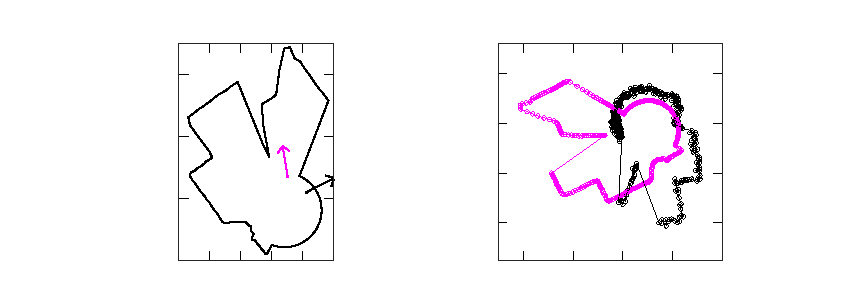
\includegraphics{./figures/parts/02/chapters/04/sections/04/sr5_sm0_0}}%
    \gplfronttext
  \end{picture}%
\endgroup

  \end{subfigure}\\%
  \begin{center}\vspace{-0.5cm}
    \hfill \texttt{FSMSM}\vspace{-0.5cm}
  \end{center}
  \begin{framed}
    \begin{subfigure}{\linewidth}\hspace{-0.25cm}
    % GNUPLOT: LaTeX picture with Postscript
\begingroup
  \makeatletter
  \providecommand\color[2][]{%
    \GenericError{(gnuplot) \space\space\space\@spaces}{%
      Package color not loaded in conjunction with
      terminal option `colourtext'%
    }{See the gnuplot documentation for explanation.%
    }{Either use 'blacktext' in gnuplot or load the package
      color.sty in LaTeX.}%
    \renewcommand\color[2][]{}%
  }%
  \providecommand\includegraphics[2][]{%
    \GenericError{(gnuplot) \space\space\space\@spaces}{%
      Package graphicx or graphics not loaded%
    }{See the gnuplot documentation for explanation.%
    }{The gnuplot epslatex terminal needs graphicx.sty or graphics.sty.}%
    \renewcommand\includegraphics[2][]{}%
  }%
  \providecommand\rotatebox[2]{#2}%
  \@ifundefined{ifGPcolor}{%
    \newif\ifGPcolor
    \GPcolorfalse
  }{}%
  \@ifundefined{ifGPblacktext}{%
    \newif\ifGPblacktext
    \GPblacktexttrue
  }{}%
  % define a \g@addto@macro without @ in the name:
  \let\gplgaddtomacro\g@addto@macro
  % define empty templates for all commands taking text:
  \gdef\gplfronttext{}%
  \gdef\gplfronttext{}%
  \makeatother
  \ifGPblacktext
    % no textcolor at all
    \def\colorrgb#1{}%
    \def\colorgray#1{}%
  \else
    % gray or color?
    \ifGPcolor
      \def\colorrgb#1{\color[rgb]{#1}}%
      \def\colorgray#1{\color[gray]{#1}}%
      \expandafter\def\csname LTw\endcsname{\color{white}}%
      \expandafter\def\csname LTb\endcsname{\color{black}}%
      \expandafter\def\csname LTa\endcsname{\color{black}}%
      \expandafter\def\csname LT0\endcsname{\color[rgb]{1,0,0}}%
      \expandafter\def\csname LT1\endcsname{\color[rgb]{0,1,0}}%
      \expandafter\def\csname LT2\endcsname{\color[rgb]{0,0,1}}%
      \expandafter\def\csname LT3\endcsname{\color[rgb]{1,0,1}}%
      \expandafter\def\csname LT4\endcsname{\color[rgb]{0,1,1}}%
      \expandafter\def\csname LT5\endcsname{\color[rgb]{1,1,0}}%
      \expandafter\def\csname LT6\endcsname{\color[rgb]{0,0,0}}%
      \expandafter\def\csname LT7\endcsname{\color[rgb]{1,0.3,0}}%
      \expandafter\def\csname LT8\endcsname{\color[rgb]{0.5,0.5,0.5}}%
    \else
      % gray
      \def\colorrgb#1{\color{black}}%
      \def\colorgray#1{\color[gray]{#1}}%
      \expandafter\def\csname LTw\endcsname{\color{white}}%
      \expandafter\def\csname LTb\endcsname{\color{black}}%
      \expandafter\def\csname LTa\endcsname{\color{black}}%
      \expandafter\def\csname LT0\endcsname{\color{black}}%
      \expandafter\def\csname LT1\endcsname{\color{black}}%
      \expandafter\def\csname LT2\endcsname{\color{black}}%
      \expandafter\def\csname LT3\endcsname{\color{black}}%
      \expandafter\def\csname LT4\endcsname{\color{black}}%
      \expandafter\def\csname LT5\endcsname{\color{black}}%
      \expandafter\def\csname LT6\endcsname{\color{black}}%
      \expandafter\def\csname LT7\endcsname{\color{black}}%
      \expandafter\def\csname LT8\endcsname{\color{black}}%
    \fi
  \fi
    \setlength{\unitlength}{0.0500bp}%
    \ifx\gptboxheight\undefined%
      \newlength{\gptboxheight}%
      \newlength{\gptboxwidth}%
      \newsavebox{\gptboxtext}%
    \fi%
    \setlength{\fboxrule}{0.5pt}%
    \setlength{\fboxsep}{1pt}%
\begin{picture}(8000.00,7000.00)%
    \gplgaddtomacro\gplfronttext{%
    }%
    \gplgaddtomacro\gplfronttext{%
    }%
    \gplgaddtomacro\gplfronttext{%
    }%
    \gplgaddtomacro\gplfronttext{%
      \colorrgb{0.00,0.00,0.00}%
      \put(1509,7049){\makebox(0,0){\strut{}\small Περιστροφή 1}}%
    }%
    \gplgaddtomacro\gplfronttext{%
      \colorrgb{0.00,0.45,0.74}%
      \put(2381,5782){\makebox(0,0)[r]{\strut{}\scriptsize $0.4$}}%
      \colorrgb{0.00,0.45,0.74}%
      \put(2381,6011){\makebox(0,0)[r]{\strut{}\scriptsize $0.6$}}%
      \colorrgb{0.00,0.45,0.74}%
      \put(2381,6241){\makebox(0,0)[r]{\strut{}\scriptsize $0.8$}}%
      \colorrgb{0.00,0.45,0.74}%
      \put(2381,6470){\makebox(0,0)[r]{\strut{}\scriptsize $1.0$}}%
      \colorrgb{0.00,0.45,0.74}%
      \put(2381,6700){\makebox(0,0)[r]{\strut{}\scriptsize $1.2$}}%
      \colorrgb{0.00,0.45,0.74}%
      \put(2381,6929){\makebox(0,0)[r]{\strut{}\scriptsize $1.4$}}%
      \colorrgb{0.15,0.15,0.15}%
      \put(2413,5662){\makebox(0,0){\strut{}\scriptsize $0$}}%
      \colorrgb{0.15,0.15,0.15}%
      \put(3739,5662){\makebox(0,0){\strut{}\scriptsize $0.5$}}%
    }%
    \gplgaddtomacro\gplfronttext{%
    }%
    \gplgaddtomacro\gplfronttext{%
      \colorrgb{0.85,0.33,0.10}%
      \put(3771,6069){\makebox(0,0)[l]{\strut{}\scriptsize $150$}}%
      \colorrgb{0.85,0.33,0.10}%
      \put(3771,6547){\makebox(0,0)[l]{\strut{}\scriptsize $200$}}%
    }%
    \gplgaddtomacro\gplfronttext{%
    }%
    \gplgaddtomacro\gplfronttext{%
    }%
    \gplgaddtomacro\gplfronttext{%
    }%
    \gplgaddtomacro\gplfronttext{%
    }%
    \gplgaddtomacro\gplfronttext{%
      \colorrgb{0.00,0.00,0.00}%
      \put(5489,7049){\makebox(0,0){\strut{}\small Μετατόπιση 1}}%
    }%
    \gplgaddtomacro\gplfronttext{%
      \colorrgb{0.00,0.45,0.74}%
      \put(6501,5782){\makebox(0,0)[r]{\strut{}\scriptsize $0.2$}}%
      \colorrgb{0.00,0.45,0.74}%
      \put(6501,5973){\makebox(0,0)[r]{\strut{}\scriptsize $0.4$}}%
      \colorrgb{0.00,0.45,0.74}%
      \put(6501,6164){\makebox(0,0)[r]{\strut{}\scriptsize $0.6$}}%
      \colorrgb{0.00,0.45,0.74}%
      \put(6501,6356){\makebox(0,0)[r]{\strut{}\scriptsize $0.8$}}%
      \colorrgb{0.00,0.45,0.74}%
      \put(6501,6547){\makebox(0,0)[r]{\strut{}\scriptsize $1.0$}}%
      \colorrgb{0.00,0.45,0.74}%
      \put(6501,6738){\makebox(0,0)[r]{\strut{}\scriptsize $1.2$}}%
      \colorrgb{0.00,0.45,0.74}%
      \put(6501,6929){\makebox(0,0)[r]{\strut{}\scriptsize $1.4$}}%
      \colorrgb{0.15,0.15,0.15}%
      \put(6633,5662){\makebox(0,0){\strut{}\scriptsize $0$}}%
      \colorrgb{0.15,0.15,0.15}%
      \put(7959,5662){\makebox(0,0){\strut{}\scriptsize $1$}}%
    }%
    \gplgaddtomacro\gplfronttext{%
    }%
    \gplgaddtomacro\gplfronttext{%
      \colorrgb{0.85,0.33,0.10}%
      \put(7991,5782){\makebox(0,0)[l]{\strut{}\scriptsize $50$}}%
      \colorrgb{0.85,0.33,0.10}%
      \put(7991,6069){\makebox(0,0)[l]{\strut{}\scriptsize $100$}}%
      \colorrgb{0.85,0.33,0.10}%
      \put(7991,6356){\makebox(0,0)[l]{\strut{}\scriptsize $150$}}%
      \colorrgb{0.85,0.33,0.10}%
      \put(7991,6642){\makebox(0,0)[l]{\strut{}\scriptsize $200$}}%
      \colorrgb{0.85,0.33,0.10}%
      \put(7991,6929){\makebox(0,0)[l]{\strut{}\scriptsize $250$}}%
    }%
    \gplgaddtomacro\gplfronttext{%
    }%
    \gplgaddtomacro\gplfronttext{%
    }%
    \gplgaddtomacro\gplfronttext{%
    }%
    \gplgaddtomacro\gplfronttext{%
    }%
    \gplgaddtomacro\gplfronttext{%
      \colorrgb{0.00,0.00,0.00}%
      \put(1429,5621){\makebox(0,0){\strut{}\small Περιστροφή 3}}%
    }%
    \gplgaddtomacro\gplfronttext{%
      \colorrgb{0.00,0.45,0.74}%
      \put(2381,4354){\makebox(0,0)[r]{\strut{}\scriptsize $0.0$}}%
      \colorrgb{0.00,0.45,0.74}%
      \put(2381,4518){\makebox(0,0)[r]{\strut{}\scriptsize $0.2$}}%
      \colorrgb{0.00,0.45,0.74}%
      \put(2381,4682){\makebox(0,0)[r]{\strut{}\scriptsize $0.4$}}%
      \colorrgb{0.00,0.45,0.74}%
      \put(2381,4846){\makebox(0,0)[r]{\strut{}\scriptsize $0.6$}}%
      \colorrgb{0.00,0.45,0.74}%
      \put(2381,5009){\makebox(0,0)[r]{\strut{}\scriptsize $0.8$}}%
      \colorrgb{0.00,0.45,0.74}%
      \put(2381,5173){\makebox(0,0)[r]{\strut{}\scriptsize $1.0$}}%
      \colorrgb{0.00,0.45,0.74}%
      \put(2381,5337){\makebox(0,0)[r]{\strut{}\scriptsize $1.2$}}%
      \colorrgb{0.00,0.45,0.74}%
      \put(2381,5501){\makebox(0,0)[r]{\strut{}\scriptsize $1.4$}}%
      \colorrgb{0.15,0.15,0.15}%
      \put(2413,4234){\makebox(0,0){\strut{}\scriptsize $0$}}%
      \colorrgb{0.15,0.15,0.15}%
      \put(2943,4234){\makebox(0,0){\strut{}\scriptsize $1$}}%
      \colorrgb{0.15,0.15,0.15}%
      \put(3474,4234){\makebox(0,0){\strut{}\scriptsize $2$}}%
    }%
    \gplgaddtomacro\gplfronttext{%
    }%
    \gplgaddtomacro\gplfronttext{%
      \colorrgb{0.85,0.33,0.10}%
      \put(3771,4354){\makebox(0,0)[l]{\strut{}\scriptsize $0$}}%
      \colorrgb{0.85,0.33,0.10}%
      \put(3771,4583){\makebox(0,0)[l]{\strut{}\scriptsize $50$}}%
      \colorrgb{0.85,0.33,0.10}%
      \put(3771,4813){\makebox(0,0)[l]{\strut{}\scriptsize $100$}}%
      \colorrgb{0.85,0.33,0.10}%
      \put(3771,5042){\makebox(0,0)[l]{\strut{}\scriptsize $150$}}%
      \colorrgb{0.85,0.33,0.10}%
      \put(3771,5272){\makebox(0,0)[l]{\strut{}\scriptsize $200$}}%
      \colorrgb{0.85,0.33,0.10}%
      \put(3771,5501){\makebox(0,0)[l]{\strut{}\scriptsize $250$}}%
    }%
    \gplgaddtomacro\gplfronttext{%
    }%
    \gplgaddtomacro\gplfronttext{%
    }%
    \gplgaddtomacro\gplfronttext{%
    }%
    \gplgaddtomacro\gplfronttext{%
    }%
    \gplgaddtomacro\gplfronttext{%
      \colorrgb{0.00,0.00,0.00}%
      \put(5529,5621){\makebox(0,0){\strut{}\small Μετατόπιση 3}}%
    }%
    \gplgaddtomacro\gplfronttext{%
      \colorrgb{0.00,0.45,0.74}%
      \put(6601,4354){\makebox(0,0)[r]{\strut{}\scriptsize $0.0$}}%
      \colorrgb{0.00,0.45,0.74}%
      \put(6601,4518){\makebox(0,0)[r]{\strut{}\scriptsize $0.2$}}%
      \colorrgb{0.00,0.45,0.74}%
      \put(6601,4682){\makebox(0,0)[r]{\strut{}\scriptsize $0.4$}}%
      \colorrgb{0.00,0.45,0.74}%
      \put(6601,4846){\makebox(0,0)[r]{\strut{}\scriptsize $0.6$}}%
      \colorrgb{0.00,0.45,0.74}%
      \put(6601,5009){\makebox(0,0)[r]{\strut{}\scriptsize $0.8$}}%
      \colorrgb{0.00,0.45,0.74}%
      \put(6601,5173){\makebox(0,0)[r]{\strut{}\scriptsize $1.0$}}%
      \colorrgb{0.00,0.45,0.74}%
      \put(6601,5337){\makebox(0,0)[r]{\strut{}\scriptsize $1.2$}}%
      \colorrgb{0.00,0.45,0.74}%
      \put(6601,5501){\makebox(0,0)[r]{\strut{}\scriptsize $1.4$}}%
      \colorrgb{0.15,0.15,0.15}%
      \put(6633,4234){\makebox(0,0){\strut{}\scriptsize $0$}}%
      \colorrgb{0.15,0.15,0.15}%
      \put(7075,4234){\makebox(0,0){\strut{}\scriptsize $1$}}%
      \colorrgb{0.15,0.15,0.15}%
      \put(7517,4234){\makebox(0,0){\strut{}\scriptsize $2$}}%
      \colorrgb{0.15,0.15,0.15}%
      \put(7959,4234){\makebox(0,0){\strut{}\scriptsize $3$}}%
    }%
    \gplgaddtomacro\gplfronttext{%
    }%
    \gplgaddtomacro\gplfronttext{%
      \colorrgb{0.85,0.33,0.10}%
      \put(7991,4354){\makebox(0,0)[l]{\strut{}\scriptsize $0$}}%
      \colorrgb{0.85,0.33,0.10}%
      \put(7991,4583){\makebox(0,0)[l]{\strut{}\scriptsize $50$}}%
      \colorrgb{0.85,0.33,0.10}%
      \put(7991,4813){\makebox(0,0)[l]{\strut{}\scriptsize $100$}}%
      \colorrgb{0.85,0.33,0.10}%
      \put(7991,5042){\makebox(0,0)[l]{\strut{}\scriptsize $150$}}%
      \colorrgb{0.85,0.33,0.10}%
      \put(7991,5272){\makebox(0,0)[l]{\strut{}\scriptsize $200$}}%
      \colorrgb{0.85,0.33,0.10}%
      \put(7991,5501){\makebox(0,0)[l]{\strut{}\scriptsize $250$}}%
    }%
    \gplgaddtomacro\gplfronttext{%
    }%
    \gplgaddtomacro\gplfronttext{%
    }%
    \gplgaddtomacro\gplfronttext{%
    }%
    \gplgaddtomacro\gplfronttext{%
    }%
    \gplgaddtomacro\gplfronttext{%
      \colorrgb{0.00,0.00,0.00}%
      \put(1429,4193){\makebox(0,0){\strut{}\small Περιστροφή 5}}%
    }%
    \gplgaddtomacro\gplfronttext{%
      \colorrgb{0.00,0.45,0.74}%
      \put(2381,2926){\makebox(0,0)[r]{\strut{}\scriptsize $0.0$}}%
      \colorrgb{0.00,0.45,0.74}%
      \put(2381,3090){\makebox(0,0)[r]{\strut{}\scriptsize $0.2$}}%
      \colorrgb{0.00,0.45,0.74}%
      \put(2381,3254){\makebox(0,0)[r]{\strut{}\scriptsize $0.4$}}%
      \colorrgb{0.00,0.45,0.74}%
      \put(2381,3418){\makebox(0,0)[r]{\strut{}\scriptsize $0.6$}}%
      \colorrgb{0.00,0.45,0.74}%
      \put(2381,3581){\makebox(0,0)[r]{\strut{}\scriptsize $0.8$}}%
      \colorrgb{0.00,0.45,0.74}%
      \put(2381,3745){\makebox(0,0)[r]{\strut{}\scriptsize $1.0$}}%
      \colorrgb{0.00,0.45,0.74}%
      \put(2381,3909){\makebox(0,0)[r]{\strut{}\scriptsize $1.2$}}%
      \colorrgb{0.00,0.45,0.74}%
      \put(2381,4073){\makebox(0,0)[r]{\strut{}\scriptsize $1.4$}}%
      \colorrgb{0.15,0.15,0.15}%
      \put(2413,2806){\makebox(0,0){\strut{}\scriptsize $0$}}%
      \colorrgb{0.15,0.15,0.15}%
      \put(2708,2806){\makebox(0,0){\strut{}\scriptsize $1$}}%
      \colorrgb{0.15,0.15,0.15}%
      \put(3002,2806){\makebox(0,0){\strut{}\scriptsize $2$}}%
      \colorrgb{0.15,0.15,0.15}%
      \put(3297,2806){\makebox(0,0){\strut{}\scriptsize $3$}}%
      \colorrgb{0.15,0.15,0.15}%
      \put(3592,2806){\makebox(0,0){\strut{}\scriptsize $4$}}%
    }%
    \gplgaddtomacro\gplfronttext{%
    }%
    \gplgaddtomacro\gplfronttext{%
      \colorrgb{0.85,0.33,0.10}%
      \put(3771,2926){\makebox(0,0)[l]{\strut{}\scriptsize $0$}}%
      \colorrgb{0.85,0.33,0.10}%
      \put(3771,3155){\makebox(0,0)[l]{\strut{}\scriptsize $50$}}%
      \colorrgb{0.85,0.33,0.10}%
      \put(3771,3385){\makebox(0,0)[l]{\strut{}\scriptsize $100$}}%
      \colorrgb{0.85,0.33,0.10}%
      \put(3771,3614){\makebox(0,0)[l]{\strut{}\scriptsize $150$}}%
      \colorrgb{0.85,0.33,0.10}%
      \put(3771,3844){\makebox(0,0)[l]{\strut{}\scriptsize $200$}}%
      \colorrgb{0.85,0.33,0.10}%
      \put(3771,4073){\makebox(0,0)[l]{\strut{}\scriptsize $250$}}%
    }%
    \gplgaddtomacro\gplfronttext{%
    }%
    \gplgaddtomacro\gplfronttext{%
    }%
    \gplgaddtomacro\gplfronttext{%
    }%
    \gplgaddtomacro\gplfronttext{%
    }%
    \gplgaddtomacro\gplfronttext{%
      \colorrgb{0.00,0.00,0.00}%
      \put(5489,4193){\makebox(0,0){\strut{}\small Μετατόπιση 5}}%
    }%
    \gplgaddtomacro\gplfronttext{%
      \colorrgb{0.00,0.45,0.74}%
      \put(6601,2926){\makebox(0,0)[r]{\strut{}\scriptsize $0.0$}}%
      \colorrgb{0.00,0.45,0.74}%
      \put(6601,3090){\makebox(0,0)[r]{\strut{}\scriptsize $0.2$}}%
      \colorrgb{0.00,0.45,0.74}%
      \put(6601,3254){\makebox(0,0)[r]{\strut{}\scriptsize $0.4$}}%
      \colorrgb{0.00,0.45,0.74}%
      \put(6601,3418){\makebox(0,0)[r]{\strut{}\scriptsize $0.6$}}%
      \colorrgb{0.00,0.45,0.74}%
      \put(6601,3581){\makebox(0,0)[r]{\strut{}\scriptsize $0.8$}}%
      \colorrgb{0.00,0.45,0.74}%
      \put(6601,3745){\makebox(0,0)[r]{\strut{}\scriptsize $1.0$}}%
      \colorrgb{0.00,0.45,0.74}%
      \put(6601,3909){\makebox(0,0)[r]{\strut{}\scriptsize $1.2$}}%
      \colorrgb{0.00,0.45,0.74}%
      \put(6601,4073){\makebox(0,0)[r]{\strut{}\scriptsize $1.4$}}%
      \colorrgb{0.15,0.15,0.15}%
      \put(6633,2806){\makebox(0,0){\strut{}\scriptsize $0$}}%
      \colorrgb{0.15,0.15,0.15}%
      \put(6898,2806){\makebox(0,0){\strut{}\scriptsize $1$}}%
      \colorrgb{0.15,0.15,0.15}%
      \put(7163,2806){\makebox(0,0){\strut{}\scriptsize $2$}}%
      \colorrgb{0.15,0.15,0.15}%
      \put(7429,2806){\makebox(0,0){\strut{}\scriptsize $3$}}%
      \colorrgb{0.15,0.15,0.15}%
      \put(7694,2806){\makebox(0,0){\strut{}\scriptsize $4$}}%
      \colorrgb{0.15,0.15,0.15}%
      \put(7959,2806){\makebox(0,0){\strut{}\scriptsize $5$}}%
    }%
    \gplgaddtomacro\gplfronttext{%
    }%
    \gplgaddtomacro\gplfronttext{%
      \colorrgb{0.85,0.33,0.10}%
      \put(7991,2926){\makebox(0,0)[l]{\strut{}\scriptsize $0$}}%
      \colorrgb{0.85,0.33,0.10}%
      \put(7991,3155){\makebox(0,0)[l]{\strut{}\scriptsize $50$}}%
      \colorrgb{0.85,0.33,0.10}%
      \put(7991,3385){\makebox(0,0)[l]{\strut{}\scriptsize $100$}}%
      \colorrgb{0.85,0.33,0.10}%
      \put(7991,3614){\makebox(0,0)[l]{\strut{}\scriptsize $150$}}%
      \colorrgb{0.85,0.33,0.10}%
      \put(7991,3844){\makebox(0,0)[l]{\strut{}\scriptsize $200$}}%
      \colorrgb{0.85,0.33,0.10}%
      \put(7991,4073){\makebox(0,0)[l]{\strut{}\scriptsize $250$}}%
    }%
    \gplgaddtomacro\gplfronttext{%
    }%
    \gplgaddtomacro\gplfronttext{%
    }%
    \gplgaddtomacro\gplfronttext{%
    }%
    \gplgaddtomacro\gplfronttext{%
    }%
    \gplgaddtomacro\gplfronttext{%
      \colorrgb{0.00,0.00,0.00}%
      \put(1429,2765){\makebox(0,0){\strut{}\small Περιστροφή 8}}%
    }%
    \gplgaddtomacro\gplfronttext{%
      \colorrgb{0.00,0.45,0.74}%
      \put(2381,1498){\makebox(0,0)[r]{\strut{}\scriptsize $0.0$}}%
      \colorrgb{0.00,0.45,0.74}%
      \put(2381,1662){\makebox(0,0)[r]{\strut{}\scriptsize $0.2$}}%
      \colorrgb{0.00,0.45,0.74}%
      \put(2381,1826){\makebox(0,0)[r]{\strut{}\scriptsize $0.4$}}%
      \colorrgb{0.00,0.45,0.74}%
      \put(2381,1990){\makebox(0,0)[r]{\strut{}\scriptsize $0.6$}}%
      \colorrgb{0.00,0.45,0.74}%
      \put(2381,2153){\makebox(0,0)[r]{\strut{}\scriptsize $0.8$}}%
      \colorrgb{0.00,0.45,0.74}%
      \put(2381,2317){\makebox(0,0)[r]{\strut{}\scriptsize $1.0$}}%
      \colorrgb{0.00,0.45,0.74}%
      \put(2381,2481){\makebox(0,0)[r]{\strut{}\scriptsize $1.2$}}%
      \colorrgb{0.00,0.45,0.74}%
      \put(2381,2645){\makebox(0,0)[r]{\strut{}\scriptsize $1.4$}}%
      \colorrgb{0.15,0.15,0.15}%
      \put(2413,1378){\makebox(0,0){\strut{}\scriptsize $0$}}%
      \colorrgb{0.15,0.15,0.15}%
      \put(2767,1378){\makebox(0,0){\strut{}\scriptsize $2$}}%
      \colorrgb{0.15,0.15,0.15}%
      \put(3120,1378){\makebox(0,0){\strut{}\scriptsize $4$}}%
      \colorrgb{0.15,0.15,0.15}%
      \put(3474,1378){\makebox(0,0){\strut{}\scriptsize $6$}}%
    }%
    \gplgaddtomacro\gplfronttext{%
    }%
    \gplgaddtomacro\gplfronttext{%
      \colorrgb{0.85,0.33,0.10}%
      \put(3771,1498){\makebox(0,0)[l]{\strut{}\scriptsize $0$}}%
      \colorrgb{0.85,0.33,0.10}%
      \put(3771,1727){\makebox(0,0)[l]{\strut{}\scriptsize $50$}}%
      \colorrgb{0.85,0.33,0.10}%
      \put(3771,1957){\makebox(0,0)[l]{\strut{}\scriptsize $100$}}%
      \colorrgb{0.85,0.33,0.10}%
      \put(3771,2186){\makebox(0,0)[l]{\strut{}\scriptsize $150$}}%
      \colorrgb{0.85,0.33,0.10}%
      \put(3771,2416){\makebox(0,0)[l]{\strut{}\scriptsize $200$}}%
      \colorrgb{0.85,0.33,0.10}%
      \put(3771,2645){\makebox(0,0)[l]{\strut{}\scriptsize $250$}}%
    }%
    \gplgaddtomacro\gplfronttext{%
    }%
    \gplgaddtomacro\gplfronttext{%
    }%
    \gplgaddtomacro\gplfronttext{%
    }%
    \gplgaddtomacro\gplfronttext{%
    }%
    \gplgaddtomacro\gplfronttext{%
      \colorrgb{0.00,0.00,0.00}%
      \put(5489,2765){\makebox(0,0){\strut{}\small Μετατόπιση 8}}%
    }%
    \gplgaddtomacro\gplfronttext{%
      \colorrgb{0.00,0.45,0.74}%
      \put(6601,1498){\makebox(0,0)[r]{\strut{}\scriptsize $0.0$}}%
      \colorrgb{0.00,0.45,0.74}%
      \put(6601,1662){\makebox(0,0)[r]{\strut{}\scriptsize $0.2$}}%
      \colorrgb{0.00,0.45,0.74}%
      \put(6601,1826){\makebox(0,0)[r]{\strut{}\scriptsize $0.4$}}%
      \colorrgb{0.00,0.45,0.74}%
      \put(6601,1990){\makebox(0,0)[r]{\strut{}\scriptsize $0.6$}}%
      \colorrgb{0.00,0.45,0.74}%
      \put(6601,2153){\makebox(0,0)[r]{\strut{}\scriptsize $0.8$}}%
      \colorrgb{0.00,0.45,0.74}%
      \put(6601,2317){\makebox(0,0)[r]{\strut{}\scriptsize $1.0$}}%
      \colorrgb{0.00,0.45,0.74}%
      \put(6601,2481){\makebox(0,0)[r]{\strut{}\scriptsize $1.2$}}%
      \colorrgb{0.00,0.45,0.74}%
      \put(6601,2645){\makebox(0,0)[r]{\strut{}\scriptsize $1.4$}}%
      \colorrgb{0.15,0.15,0.15}%
      \put(6633,1378){\makebox(0,0){\strut{}\scriptsize $0$}}%
      \colorrgb{0.15,0.15,0.15}%
      \put(6965,1378){\makebox(0,0){\strut{}\scriptsize $2$}}%
      \colorrgb{0.15,0.15,0.15}%
      \put(7296,1378){\makebox(0,0){\strut{}\scriptsize $4$}}%
      \colorrgb{0.15,0.15,0.15}%
      \put(7628,1378){\makebox(0,0){\strut{}\scriptsize $6$}}%
      \colorrgb{0.15,0.15,0.15}%
      \put(7959,1378){\makebox(0,0){\strut{}\scriptsize $8$}}%
    }%
    \gplgaddtomacro\gplfronttext{%
    }%
    \gplgaddtomacro\gplfronttext{%
      \colorrgb{0.85,0.33,0.10}%
      \put(7991,1498){\makebox(0,0)[l]{\strut{}\scriptsize $0$}}%
      \colorrgb{0.85,0.33,0.10}%
      \put(7991,1727){\makebox(0,0)[l]{\strut{}\scriptsize $50$}}%
      \colorrgb{0.85,0.33,0.10}%
      \put(7991,1957){\makebox(0,0)[l]{\strut{}\scriptsize $100$}}%
      \colorrgb{0.85,0.33,0.10}%
      \put(7991,2186){\makebox(0,0)[l]{\strut{}\scriptsize $150$}}%
      \colorrgb{0.85,0.33,0.10}%
      \put(7991,2416){\makebox(0,0)[l]{\strut{}\scriptsize $200$}}%
      \colorrgb{0.85,0.33,0.10}%
      \put(7991,2645){\makebox(0,0)[l]{\strut{}\scriptsize $250$}}%
    }%
    \gplgaddtomacro\gplfronttext{%
    }%
    \gplgaddtomacro\gplfronttext{%
    }%
    \gplgaddtomacro\gplfronttext{%
    }%
    \gplgaddtomacro\gplfronttext{%
    }%
    \gplgaddtomacro\gplfronttext{%
      \colorrgb{0.00,0.00,0.00}%
      \put(1429,1337){\makebox(0,0){\strut{}\small Περιστροφή 20}}%
    }%
    \gplgaddtomacro\gplfronttext{%
      \colorrgb{0.00,0.45,0.74}%
      \put(2381,70){\makebox(0,0)[r]{\strut{}\scriptsize $0.0$}}%
      \colorrgb{0.00,0.45,0.74}%
      \put(2381,234){\makebox(0,0)[r]{\strut{}\scriptsize $0.2$}}%
      \colorrgb{0.00,0.45,0.74}%
      \put(2381,398){\makebox(0,0)[r]{\strut{}\scriptsize $0.4$}}%
      \colorrgb{0.00,0.45,0.74}%
      \put(2381,562){\makebox(0,0)[r]{\strut{}\scriptsize $0.6$}}%
      \colorrgb{0.00,0.45,0.74}%
      \put(2381,725){\makebox(0,0)[r]{\strut{}\scriptsize $0.8$}}%
      \colorrgb{0.00,0.45,0.74}%
      \put(2381,889){\makebox(0,0)[r]{\strut{}\scriptsize $1.0$}}%
      \colorrgb{0.00,0.45,0.74}%
      \put(2381,1053){\makebox(0,0)[r]{\strut{}\scriptsize $1.2$}}%
      \colorrgb{0.00,0.45,0.74}%
      \put(2381,1217){\makebox(0,0)[r]{\strut{}\scriptsize $1.4$}}%
      \colorrgb{0.15,0.15,0.15}%
      \put(2413,-50){\makebox(0,0){\strut{}\scriptsize $0$}}%
      \colorrgb{0.15,0.15,0.15}%
      \put(2753,-50){\makebox(0,0){\strut{}\scriptsize $5$}}%
      \colorrgb{0.15,0.15,0.15}%
      \put(3093,-50){\makebox(0,0){\strut{}\scriptsize $10$}}%
      \colorrgb{0.15,0.15,0.15}%
      \put(3433,-50){\makebox(0,0){\strut{}\scriptsize $15$}}%
    }%
    \gplgaddtomacro\gplfronttext{%
    }%
    \gplgaddtomacro\gplfronttext{%
      \colorrgb{0.85,0.33,0.10}%
      \put(3771,70){\makebox(0,0)[l]{\strut{}\scriptsize $0$}}%
      \colorrgb{0.85,0.33,0.10}%
      \put(3771,299){\makebox(0,0)[l]{\strut{}\scriptsize $50$}}%
      \colorrgb{0.85,0.33,0.10}%
      \put(3771,529){\makebox(0,0)[l]{\strut{}\scriptsize $100$}}%
      \colorrgb{0.85,0.33,0.10}%
      \put(3771,758){\makebox(0,0)[l]{\strut{}\scriptsize $150$}}%
      \colorrgb{0.85,0.33,0.10}%
      \put(3771,988){\makebox(0,0)[l]{\strut{}\scriptsize $200$}}%
      \colorrgb{0.85,0.33,0.10}%
      \put(3771,1217){\makebox(0,0)[l]{\strut{}\scriptsize $250$}}%
    }%
    \gplgaddtomacro\gplfronttext{%
    }%
    \gplgaddtomacro\gplfronttext{%
    }%
    \gplgaddtomacro\gplfronttext{%
    }%
    \gplgaddtomacro\gplfronttext{%
    }%
    \gplgaddtomacro\gplfronttext{%
      \colorrgb{0.00,0.00,0.00}%
      \put(5489,1337){\makebox(0,0){\strut{}\small Μετατόπιση 20}}%
    }%
    \gplgaddtomacro\gplfronttext{%
      \colorrgb{0.00,0.45,0.74}%
      \put(6601,70){\makebox(0,0)[r]{\strut{}\scriptsize $0.0$}}%
      \colorrgb{0.00,0.45,0.74}%
      \put(6601,234){\makebox(0,0)[r]{\strut{}\scriptsize $0.2$}}%
      \colorrgb{0.00,0.45,0.74}%
      \put(6601,398){\makebox(0,0)[r]{\strut{}\scriptsize $0.4$}}%
      \colorrgb{0.00,0.45,0.74}%
      \put(6601,562){\makebox(0,0)[r]{\strut{}\scriptsize $0.6$}}%
      \colorrgb{0.00,0.45,0.74}%
      \put(6601,725){\makebox(0,0)[r]{\strut{}\scriptsize $0.8$}}%
      \colorrgb{0.00,0.45,0.74}%
      \put(6601,889){\makebox(0,0)[r]{\strut{}\scriptsize $1.0$}}%
      \colorrgb{0.00,0.45,0.74}%
      \put(6601,1053){\makebox(0,0)[r]{\strut{}\scriptsize $1.2$}}%
      \colorrgb{0.00,0.45,0.74}%
      \put(6601,1217){\makebox(0,0)[r]{\strut{}\scriptsize $1.4$}}%
      \colorrgb{0.15,0.15,0.15}%
      \put(6633,-50){\makebox(0,0){\strut{}\scriptsize $0$}}%
      \colorrgb{0.15,0.15,0.15}%
      \put(6965,-50){\makebox(0,0){\strut{}\scriptsize $5$}}%
      \colorrgb{0.15,0.15,0.15}%
      \put(7296,-50){\makebox(0,0){\strut{}\scriptsize $10$}}%
      \colorrgb{0.15,0.15,0.15}%
      \put(7628,-50){\makebox(0,0){\strut{}\scriptsize $15$}}%
      \colorrgb{0.15,0.15,0.15}%
      \put(7959,-50){\makebox(0,0){\strut{}\scriptsize $20$}}%
    }%
    \gplgaddtomacro\gplfronttext{%
    }%
    \gplgaddtomacro\gplfronttext{%
      \colorrgb{0.85,0.33,0.10}%
      \put(7991,70){\makebox(0,0)[l]{\strut{}\scriptsize $0$}}%
      \colorrgb{0.85,0.33,0.10}%
      \put(7991,299){\makebox(0,0)[l]{\strut{}\scriptsize $50$}}%
      \colorrgb{0.85,0.33,0.10}%
      \put(7991,529){\makebox(0,0)[l]{\strut{}\scriptsize $100$}}%
      \colorrgb{0.85,0.33,0.10}%
      \put(7991,758){\makebox(0,0)[l]{\strut{}\scriptsize $150$}}%
      \colorrgb{0.85,0.33,0.10}%
      \put(7991,988){\makebox(0,0)[l]{\strut{}\scriptsize $200$}}%
      \colorrgb{0.85,0.33,0.10}%
      \put(7991,1217){\makebox(0,0)[l]{\strut{}\scriptsize $250$}}%
    }%
    \gplgaddtomacro\gplfronttext{%
    }%
    \put(0,0){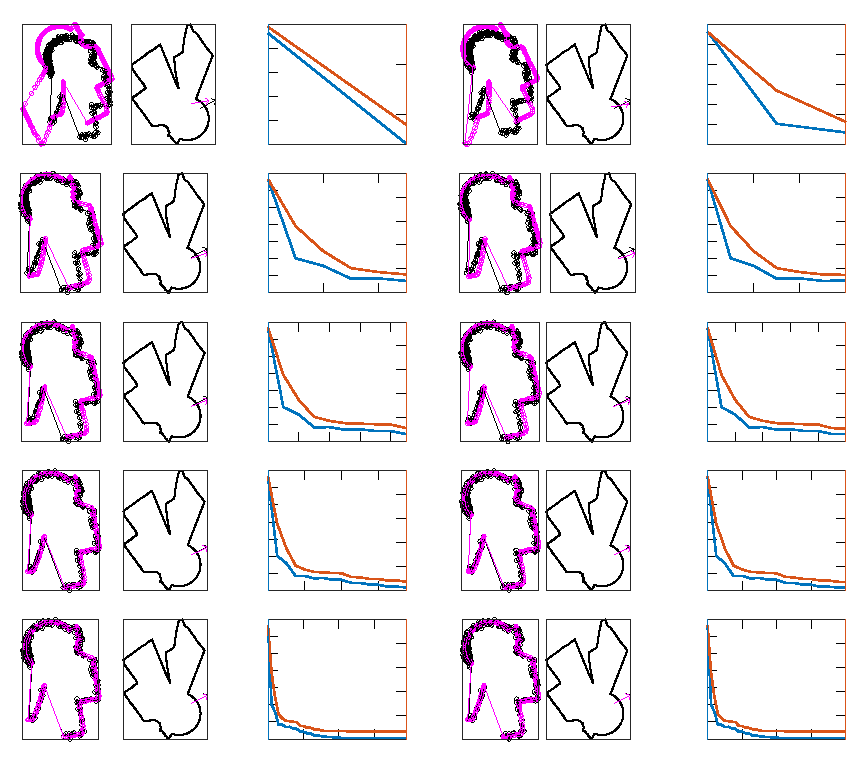
\includegraphics{./figures/parts/02/chapters/04/sections/04/sr5_sm0_1}}%
    \gplfronttext
  \end{picture}%
\endgroup

    \end{subfigure}\\%
  \end{framed}
  \begin{subfigure}{\linewidth}\hspace{-0.25cm}
    % GNUPLOT: LaTeX picture with Postscript
\begingroup
  \makeatletter
  \providecommand\color[2][]{%
    \GenericError{(gnuplot) \space\space\space\@spaces}{%
      Package color not loaded in conjunction with
      terminal option `colourtext'%
    }{See the gnuplot documentation for explanation.%
    }{Either use 'blacktext' in gnuplot or load the package
      color.sty in LaTeX.}%
    \renewcommand\color[2][]{}%
  }%
  \providecommand\includegraphics[2][]{%
    \GenericError{(gnuplot) \space\space\space\@spaces}{%
      Package graphicx or graphics not loaded%
    }{See the gnuplot documentation for explanation.%
    }{The gnuplot epslatex terminal needs graphicx.sty or graphics.sty.}%
    \renewcommand\includegraphics[2][]{}%
  }%
  \providecommand\rotatebox[2]{#2}%
  \@ifundefined{ifGPcolor}{%
    \newif\ifGPcolor
    \GPcolorfalse
  }{}%
  \@ifundefined{ifGPblacktext}{%
    \newif\ifGPblacktext
    \GPblacktexttrue
  }{}%
  % define a \g@addto@macro without @ in the name:
  \let\gplgaddtomacro\g@addto@macro
  % define empty templates for all commands taking text:
  \gdef\gplfronttext{}%
  \gdef\gplfronttext{}%
  \makeatother
  \ifGPblacktext
    % no textcolor at all
    \def\colorrgb#1{}%
    \def\colorgray#1{}%
  \else
    % gray or color?
    \ifGPcolor
      \def\colorrgb#1{\color[rgb]{#1}}%
      \def\colorgray#1{\color[gray]{#1}}%
      \expandafter\def\csname LTw\endcsname{\color{white}}%
      \expandafter\def\csname LTb\endcsname{\color{black}}%
      \expandafter\def\csname LTa\endcsname{\color{black}}%
      \expandafter\def\csname LT0\endcsname{\color[rgb]{1,0,0}}%
      \expandafter\def\csname LT1\endcsname{\color[rgb]{0,1,0}}%
      \expandafter\def\csname LT2\endcsname{\color[rgb]{0,0,1}}%
      \expandafter\def\csname LT3\endcsname{\color[rgb]{1,0,1}}%
      \expandafter\def\csname LT4\endcsname{\color[rgb]{0,1,1}}%
      \expandafter\def\csname LT5\endcsname{\color[rgb]{1,1,0}}%
      \expandafter\def\csname LT6\endcsname{\color[rgb]{0,0,0}}%
      \expandafter\def\csname LT7\endcsname{\color[rgb]{1,0.3,0}}%
      \expandafter\def\csname LT8\endcsname{\color[rgb]{0.5,0.5,0.5}}%
    \else
      % gray
      \def\colorrgb#1{\color{black}}%
      \def\colorgray#1{\color[gray]{#1}}%
      \expandafter\def\csname LTw\endcsname{\color{white}}%
      \expandafter\def\csname LTb\endcsname{\color{black}}%
      \expandafter\def\csname LTa\endcsname{\color{black}}%
      \expandafter\def\csname LT0\endcsname{\color{black}}%
      \expandafter\def\csname LT1\endcsname{\color{black}}%
      \expandafter\def\csname LT2\endcsname{\color{black}}%
      \expandafter\def\csname LT3\endcsname{\color{black}}%
      \expandafter\def\csname LT4\endcsname{\color{black}}%
      \expandafter\def\csname LT5\endcsname{\color{black}}%
      \expandafter\def\csname LT6\endcsname{\color{black}}%
      \expandafter\def\csname LT7\endcsname{\color{black}}%
      \expandafter\def\csname LT8\endcsname{\color{black}}%
    \fi
  \fi
    \setlength{\unitlength}{0.0500bp}%
    \ifx\gptboxheight\undefined%
      \newlength{\gptboxheight}%
      \newlength{\gptboxwidth}%
      \newsavebox{\gptboxtext}%
    \fi%
    \setlength{\fboxrule}{0.5pt}%
    \setlength{\fboxsep}{1pt}%
\begin{picture}(8000.00,2600.00)%
    \gplgaddtomacro\gplfronttext{%
      \colorrgb{0.15,0.15,0.15}%
      \put(1425,260){\makebox(0,0)[r]{\strut{}$1.0$}}%
      \colorrgb{0.15,0.15,0.15}%
      \put(1425,854){\makebox(0,0)[r]{\strut{}$2.0$}}%
      \colorrgb{0.15,0.15,0.15}%
      \put(1425,1448){\makebox(0,0)[r]{\strut{}$3.0$}}%
      \colorrgb{0.15,0.15,0.15}%
      \put(1425,2042){\makebox(0,0)[r]{\strut{}$4.0$}}%
      \colorrgb{0.15,0.15,0.15}%
      \put(1854,40){\makebox(0,0){\strut{}$-1.0$}}%
      \colorrgb{0.15,0.15,0.15}%
      \put(2448,40){\makebox(0,0){\strut{}$0$}}%
      \colorrgb{0.15,0.15,0.15}%
      \put(3042,40){\makebox(0,0){\strut{}$1.0$}}%
    }%
    \gplgaddtomacro\gplfronttext{%
    }%
    \gplgaddtomacro\gplfronttext{%
      \colorrgb{0.15,0.15,0.15}%
      \put(4676,557){\makebox(0,0)[r]{\strut{}$-2.0$}}%
      \colorrgb{0.15,0.15,0.15}%
      \put(4676,1151){\makebox(0,0)[r]{\strut{}$-1.0$}}%
      \colorrgb{0.15,0.15,0.15}%
      \put(4676,1745){\makebox(0,0)[r]{\strut{}$0$}}%
      \colorrgb{0.15,0.15,0.15}%
      \put(4676,2339){\makebox(0,0)[r]{\strut{}$1.0$}}%
      \colorrgb{0.15,0.15,0.15}%
      \put(4808,40){\makebox(0,0){\strut{}$-1.0$}}%
      \colorrgb{0.15,0.15,0.15}%
      \put(5402,40){\makebox(0,0){\strut{}$0$}}%
      \colorrgb{0.15,0.15,0.15}%
      \put(5996,40){\makebox(0,0){\strut{}$1.0$}}%
      \colorrgb{0.15,0.15,0.15}%
      \put(6590,40){\makebox(0,0){\strut{}$2.0$}}%
    }%
    \gplgaddtomacro\gplfronttext{%
      \put(2299,2559){\makebox(0,0){\strut{}Τελική εκτίμηση}}%
      \put(5699,2559){\makebox(0,0){\strut{}Τελική ευθυγράμμιση}}%
    }%
    \put(0,0){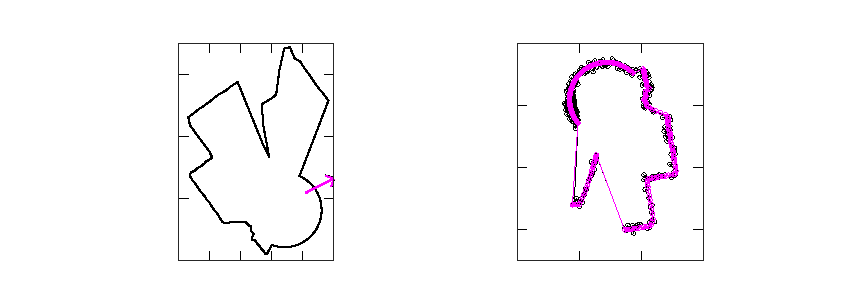
\includegraphics{./figures/parts/02/chapters/04/sections/04/sr5_sm0_2}}%
    \gplfronttext
  \end{picture}%
\endgroup

  \end{subfigure}%
  \caption{\small Παράδειγμα εξέλιξης επιτυχούς ευθυγράμμισης πραγματικής με
           εικονικές σαρώσεις μέσω της μεθόδου FSMSM. Η πραγματική στάση του
           αισθητήρα και η πραγματική σάρωση απεικονίζονται με μαύρο χρώμα, ενώ
           η εκτίμηση της στάσης και οι εικονικές σαρώσεις με ματζέντα. Τα
           διαγράμματα της τρίτης και έκτης στήλης απεικονίζουν με μπλε το
           ολικό σφάλμα εκτίμησης στάσης, και με κόκκινο την τιμή της μετρικής
           CAER}
  \label{fig:02_04_06:02}
\end{figure}

Στο σχήμα \ref{fig:02_04_06:03} παρουσιάζονται τα ίδια στοιχεία όπως και στο
σχήμα \ref{fig:02_04_06:02}, για μία ανεπιτυχή όμως ευθυγράμμιση. Εδώ η
εκτίμηση της στάσης του αισθητήρα ισούται με την πραγματική του στάση,
μετατοπισμένη όμως κατά ένα μέτρο στον οριζόντιο άξονα προς τα αριστερά. Ο
λόγος για τον οποίον η ευθυγράμμιση αποτυγχάνει είναι γιατί η εκτίμηση του
προσανατολισμού αποκλίνει κιόλας από το πρώτο βήμα, το οποίο γεγονός οφείλεται
στην αδυναμία της μεθόδου \texttt{x1} να εκτιμήσει τον προσανατολισμό της
πραγματικής στάσης του αισθητήρα, και όχι σε κάποια μη γραμμικότητα της
μετρικής CAER. Η αιτία αυτής της αδυναμίας οφείλεται στο ``μεγάλο" σφάλμα
εκτίμησης θέσης, το οποίο, όπως διακρίνεται και από το σχήμα, αλλοιώνει τη
μορφή των δύο σαρώσεων. Αυτή η αλλοίωση οφείλεται στο γεγονός ότι από
διαφορετικές θέσεις είναι εν γένει ορατές διαφορετικές περιοχές του
περιβάλλοντος.  Η επιτυχία ή αποτυχία κάθε μεθόδου εξαρτάται συνεπώς και από
την απόσταση μεταξύ της πραγματικής με την εκτιμώμενη θέση, και από το ίδιο το
περιβάλλον ως ανεξάρτητη μεταβλητή.  Αυτού του είδους τα σφάλματα ενεργούν ως
δυσχέρειες στην ευθυγράμμιση λόγω του γεγονότος ότι οι μέθοδοι εκτίμησης του
προσανατολισμού της FSMSM λειτουργούν απευθείας στο χώρο των μετρήσεων χωρίς
τον υπολογισμό αντιστοιχίσεων, σε αντίθεση με τις υπόλοιπες μεθόδους
ευθυγράμμισης που είδαμε στην προηγούμενη ενότητα. Ως αναφορά παραθέτουμε πως η
μέθοδος PLICP, στο συγκεκριμένο παράδειγμα, είναι ικανή να εκτιμήσει την
πραγματική στάση με τελικό σφάλμα εκτίμησης περίπου δύο εκατοστών.\footnote{Εδώ
πρέπει να επισημάνουμε πως η σύγκλιση σε καταστάσεις ``μεγάλων" σφαλμάτων θέσης
δεν είναι κάποιο αποκλειστικό χαρακτηριστικό των μεθόδων που χρησιμοποιούν
αντιστοιχίσεις, όπως ακριβώς και η απόκλιση δεν είναι αποκλειστικό
χαρακτηριστικό της FSMSM.  Όπως θα δούμε σε αντίστοιχο παράδειγμα στο επόμενο
κεφάλαιο (σχήμα \ref{fig:02_05_04:02}) δεν υπάρχει κάποιος ευδιάκριτος
παράγοντας που διακρίνει εκ-των-προτέρων την απόκριση των δύο οικογενειών
μεθόδων.} Τέτοιου μέτρου αρχικά σφάλματα θέσης δεν αναφέρονται στη βιβλιογραφία
(---ούτε υπάρχουν στην εμπειρία του συγγραφέα)---παρ' όλα αυτά αναφέρουμε τον
περιορισμό της μεθόδου FSMSM όσο αφορά σε τέτοια σφάλματα θέσης ως έναν
παράγοντα οριοθέτησης της απόκρισης της μεθόδου ως θεωρητικό κατασκεύασμα. Σε
αυτό το παράδειγμα παρατηρούμε πως μετά την απόκλιση της εκτίμησης
προσανατολισμού το σφάλμα εκτίμησης της θέσης αυξάνει, με αποτέλεσμα την
επιπρόσθετη επιβάρυνση του συστήματος εκτίμησης προσανατολισμού στην επόμενη
επανάληψη. Σε αυτό το σημείο η εκτίμηση στάσης έχει αποκλίνει περαιτέρω, και
έχει παγιδευτεί ες αεί σε όλως διόλου εσφαλμένη εκτίμηση. Και σε αυτήν την
περίπτωση, εάν καταγράφετο η τιμή της μετρικής CAER πριν και μετά τη διενέργεια
της ευθυγράμμισης, θα ήταν δυνατή η σύγκριση των δύο τιμών, και κατά συνέπεια η
αποφυγή, κατ' ελάχιστον, της απόκλισης της εκτίμησης.

\begin{figure}
  \begin{subfigure}{\linewidth}\centering
      % GNUPLOT: LaTeX picture with Postscript
\begingroup
  \makeatletter
  \providecommand\color[2][]{%
    \GenericError{(gnuplot) \space\space\space\@spaces}{%
      Package color not loaded in conjunction with
      terminal option `colourtext'%
    }{See the gnuplot documentation for explanation.%
    }{Either use 'blacktext' in gnuplot or load the package
      color.sty in LaTeX.}%
    \renewcommand\color[2][]{}%
  }%
  \providecommand\includegraphics[2][]{%
    \GenericError{(gnuplot) \space\space\space\@spaces}{%
      Package graphicx or graphics not loaded%
    }{See the gnuplot documentation for explanation.%
    }{The gnuplot epslatex terminal needs graphicx.sty or graphics.sty.}%
    \renewcommand\includegraphics[2][]{}%
  }%
  \providecommand\rotatebox[2]{#2}%
  \@ifundefined{ifGPcolor}{%
    \newif\ifGPcolor
    \GPcolorfalse
  }{}%
  \@ifundefined{ifGPblacktext}{%
    \newif\ifGPblacktext
    \GPblacktexttrue
  }{}%
  % define a \g@addto@macro without @ in the name:
  \let\gplgaddtomacro\g@addto@macro
  % define empty templates for all commands taking text:
  \gdef\gplfronttext{}%
  \gdef\gplfronttext{}%
  \makeatother
  \ifGPblacktext
    % no textcolor at all
    \def\colorrgb#1{}%
    \def\colorgray#1{}%
  \else
    % gray or color?
    \ifGPcolor
      \def\colorrgb#1{\color[rgb]{#1}}%
      \def\colorgray#1{\color[gray]{#1}}%
      \expandafter\def\csname LTw\endcsname{\color{white}}%
      \expandafter\def\csname LTb\endcsname{\color{black}}%
      \expandafter\def\csname LTa\endcsname{\color{black}}%
      \expandafter\def\csname LT0\endcsname{\color[rgb]{1,0,0}}%
      \expandafter\def\csname LT1\endcsname{\color[rgb]{0,1,0}}%
      \expandafter\def\csname LT2\endcsname{\color[rgb]{0,0,1}}%
      \expandafter\def\csname LT3\endcsname{\color[rgb]{1,0,1}}%
      \expandafter\def\csname LT4\endcsname{\color[rgb]{0,1,1}}%
      \expandafter\def\csname LT5\endcsname{\color[rgb]{1,1,0}}%
      \expandafter\def\csname LT6\endcsname{\color[rgb]{0,0,0}}%
      \expandafter\def\csname LT7\endcsname{\color[rgb]{1,0.3,0}}%
      \expandafter\def\csname LT8\endcsname{\color[rgb]{0.5,0.5,0.5}}%
    \else
      % gray
      \def\colorrgb#1{\color{black}}%
      \def\colorgray#1{\color[gray]{#1}}%
      \expandafter\def\csname LTw\endcsname{\color{white}}%
      \expandafter\def\csname LTb\endcsname{\color{black}}%
      \expandafter\def\csname LTa\endcsname{\color{black}}%
      \expandafter\def\csname LT0\endcsname{\color{black}}%
      \expandafter\def\csname LT1\endcsname{\color{black}}%
      \expandafter\def\csname LT2\endcsname{\color{black}}%
      \expandafter\def\csname LT3\endcsname{\color{black}}%
      \expandafter\def\csname LT4\endcsname{\color{black}}%
      \expandafter\def\csname LT5\endcsname{\color{black}}%
      \expandafter\def\csname LT6\endcsname{\color{black}}%
      \expandafter\def\csname LT7\endcsname{\color{black}}%
      \expandafter\def\csname LT8\endcsname{\color{black}}%
    \fi
  \fi
    \setlength{\unitlength}{0.0500bp}%
    \ifx\gptboxheight\undefined%
      \newlength{\gptboxheight}%
      \newlength{\gptboxwidth}%
      \newsavebox{\gptboxtext}%
    \fi%
    \setlength{\fboxrule}{0.5pt}%
    \setlength{\fboxsep}{1pt}%
\begin{picture}(6000.00,3000.00)%
    \gplgaddtomacro\gplfronttext{%
      \colorrgb{0.15,0.15,0.15}%
      \put(465,300){\makebox(0,0)[r]{\strut{}\scriptsize $1.0$}}%
      \colorrgb{0.15,0.15,0.15}%
      \put(465,985){\makebox(0,0)[r]{\strut{}\scriptsize $2.0$}}%
      \colorrgb{0.15,0.15,0.15}%
      \put(465,1671){\makebox(0,0)[r]{\strut{}\scriptsize $3.0$}}%
      \colorrgb{0.15,0.15,0.15}%
      \put(465,2356){\makebox(0,0)[r]{\strut{}\scriptsize $4.0$}}%
      \colorrgb{0.15,0.15,0.15}%
      \put(940,80){\makebox(0,0){\strut{}\scriptsize $-1$}}%
      \colorrgb{0.15,0.15,0.15}%
      \put(1625,80){\makebox(0,0){\strut{}\scriptsize $0.0$}}%
      \colorrgb{0.15,0.15,0.15}%
      \put(2311,80){\makebox(0,0){\strut{}\scriptsize $1.0$}}%
    }%
    \gplgaddtomacro\gplfronttext{%
      \colorrgb{0.00,0.00,0.00}%
      \put(1454,2919){\makebox(0,0){\strut{}Ευκλείδειος χώρος}}%
    }%
    \gplgaddtomacro\gplfronttext{%
      \colorrgb{0.15,0.15,0.15}%
      \put(3171,714){\makebox(0,0)[r]{\strut{}\scriptsize $-2.0$}}%
      \colorrgb{0.15,0.15,0.15}%
      \put(3171,1265){\makebox(0,0)[r]{\strut{}\scriptsize $-1.0$}}%
      \colorrgb{0.15,0.15,0.15}%
      \put(3171,1817){\makebox(0,0)[r]{\strut{}\scriptsize $0$}}%
      \colorrgb{0.15,0.15,0.15}%
      \put(3171,2368){\makebox(0,0)[r]{\strut{}\scriptsize $1.0$}}%
      \colorrgb{0.15,0.15,0.15}%
      \put(3579,80){\makebox(0,0){\strut{}\scriptsize $-2.0$}}%
      \colorrgb{0.15,0.15,0.15}%
      \put(4682,80){\makebox(0,0){\strut{}\scriptsize $0$}}%
      \colorrgb{0.15,0.15,0.15}%
      \put(5785,80){\makebox(0,0){\strut{}\scriptsize $2.0$}}%
    }%
    \gplgaddtomacro\gplfronttext{%
      \colorrgb{0.00,0.00,0.00}%
      \put(4544,2919){\makebox(0,0){\strut{}Μετρήσεων χώρος}}%
    }%
    \put(0,0){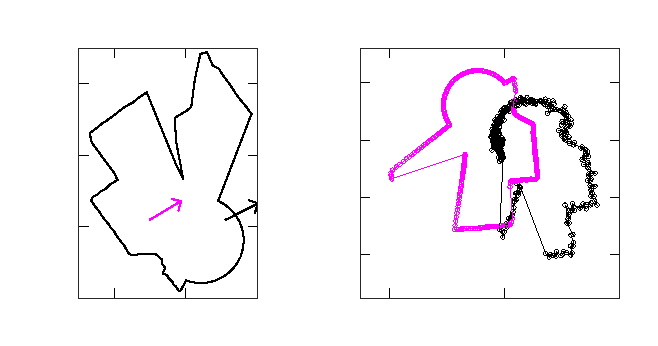
\includegraphics{./figures/parts/02/chapters/04/sections/06/sr5_sm0_fail_0}}%
    \gplfronttext
  \end{picture}%
\endgroup

    \end{subfigure}\vspace{1cm}\\
    \begin{subfigure}{\linewidth}
      % GNUPLOT: LaTeX picture with Postscript
\begingroup
  \makeatletter
  \providecommand\color[2][]{%
    \GenericError{(gnuplot) \space\space\space\@spaces}{%
      Package color not loaded in conjunction with
      terminal option `colourtext'%
    }{See the gnuplot documentation for explanation.%
    }{Either use 'blacktext' in gnuplot or load the package
      color.sty in LaTeX.}%
    \renewcommand\color[2][]{}%
  }%
  \providecommand\includegraphics[2][]{%
    \GenericError{(gnuplot) \space\space\space\@spaces}{%
      Package graphicx or graphics not loaded%
    }{See the gnuplot documentation for explanation.%
    }{The gnuplot epslatex terminal needs graphicx.sty or graphics.sty.}%
    \renewcommand\includegraphics[2][]{}%
  }%
  \providecommand\rotatebox[2]{#2}%
  \@ifundefined{ifGPcolor}{%
    \newif\ifGPcolor
    \GPcolorfalse
  }{}%
  \@ifundefined{ifGPblacktext}{%
    \newif\ifGPblacktext
    \GPblacktexttrue
  }{}%
  % define a \g@addto@macro without @ in the name:
  \let\gplgaddtomacro\g@addto@macro
  % define empty templates for all commands taking text:
  \gdef\gplfronttext{}%
  \gdef\gplfronttext{}%
  \makeatother
  \ifGPblacktext
    % no textcolor at all
    \def\colorrgb#1{}%
    \def\colorgray#1{}%
  \else
    % gray or color?
    \ifGPcolor
      \def\colorrgb#1{\color[rgb]{#1}}%
      \def\colorgray#1{\color[gray]{#1}}%
      \expandafter\def\csname LTw\endcsname{\color{white}}%
      \expandafter\def\csname LTb\endcsname{\color{black}}%
      \expandafter\def\csname LTa\endcsname{\color{black}}%
      \expandafter\def\csname LT0\endcsname{\color[rgb]{1,0,0}}%
      \expandafter\def\csname LT1\endcsname{\color[rgb]{0,1,0}}%
      \expandafter\def\csname LT2\endcsname{\color[rgb]{0,0,1}}%
      \expandafter\def\csname LT3\endcsname{\color[rgb]{1,0,1}}%
      \expandafter\def\csname LT4\endcsname{\color[rgb]{0,1,1}}%
      \expandafter\def\csname LT5\endcsname{\color[rgb]{1,1,0}}%
      \expandafter\def\csname LT6\endcsname{\color[rgb]{0,0,0}}%
      \expandafter\def\csname LT7\endcsname{\color[rgb]{1,0.3,0}}%
      \expandafter\def\csname LT8\endcsname{\color[rgb]{0.5,0.5,0.5}}%
    \else
      % gray
      \def\colorrgb#1{\color{black}}%
      \def\colorgray#1{\color[gray]{#1}}%
      \expandafter\def\csname LTw\endcsname{\color{white}}%
      \expandafter\def\csname LTb\endcsname{\color{black}}%
      \expandafter\def\csname LTa\endcsname{\color{black}}%
      \expandafter\def\csname LT0\endcsname{\color{black}}%
      \expandafter\def\csname LT1\endcsname{\color{black}}%
      \expandafter\def\csname LT2\endcsname{\color{black}}%
      \expandafter\def\csname LT3\endcsname{\color{black}}%
      \expandafter\def\csname LT4\endcsname{\color{black}}%
      \expandafter\def\csname LT5\endcsname{\color{black}}%
      \expandafter\def\csname LT6\endcsname{\color{black}}%
      \expandafter\def\csname LT7\endcsname{\color{black}}%
      \expandafter\def\csname LT8\endcsname{\color{black}}%
    \fi
  \fi
    \setlength{\unitlength}{0.0500bp}%
    \ifx\gptboxheight\undefined%
      \newlength{\gptboxheight}%
      \newlength{\gptboxwidth}%
      \newsavebox{\gptboxtext}%
    \fi%
    \setlength{\fboxrule}{0.5pt}%
    \setlength{\fboxsep}{1pt}%
\begin{picture}(8000.00,3000.00)%
    \gplgaddtomacro\gplfronttext{%
    }%
    \gplgaddtomacro\gplfronttext{%
      \colorrgb{0.00,0.00,0.00}%
      \put(623,3089){\makebox(0,0){\strut{}\small Περιστροφή 1}}%
    }%
    \gplgaddtomacro\gplfronttext{%
    }%
    \gplgaddtomacro\gplfronttext{%
    }%
    \gplgaddtomacro\gplfronttext{%
      \colorrgb{0.00,0.45,0.74}%
      \put(2541,1560){\makebox(0,0)[r]{\strut{}\scriptsize $1.0$}}%
      \colorrgb{0.00,0.45,0.74}%
      \put(2541,2265){\makebox(0,0)[r]{\strut{}\scriptsize $2.0$}}%
      \colorrgb{0.00,0.45,0.74}%
      \put(2541,2969){\makebox(0,0)[r]{\strut{}\scriptsize $3.0$}}%
      \colorrgb{0.15,0.15,0.15}%
      %\put(2573,1340){\makebox(0,0){\strut{}\scriptsize $0$}}%
      %\colorrgb{0.15,0.15,0.15}%
      %\put(3899,1340){\makebox(0,0){\strut{}\scriptsize $0.5$}}%
    }%
    \gplgaddtomacro\gplfronttext{%
    }%
    \gplgaddtomacro\gplfronttext{%
%      \colorrgb{0.85,0.33,0.10}%
      %\put(4031,1560){\makebox(0,0)[l]{\strut{}\scriptsize $100$}}%
      %\colorrgb{0.85,0.33,0.10}%
      %\put(4031,1842){\makebox(0,0)[l]{\strut{}\scriptsize $150$}}%
      %\colorrgb{0.85,0.33,0.10}%
      %\put(4031,2124){\makebox(0,0)[l]{\strut{}\scriptsize $200$}}%
      %\colorrgb{0.85,0.33,0.10}%
      %\put(4031,2405){\makebox(0,0)[l]{\strut{}\scriptsize $250$}}%
      %\colorrgb{0.85,0.33,0.10}%
      %\put(4031,2687){\makebox(0,0)[l]{\strut{}\scriptsize $300$}}%
      %\colorrgb{0.85,0.33,0.10}%
      %\put(4031,2969){\makebox(0,0)[l]{\strut{}\scriptsize $350$}}%
    }%
    \gplgaddtomacro\gplfronttext{%
    }%
    \gplgaddtomacro\gplfronttext{%
    }%
    \gplgaddtomacro\gplfronttext{%
      \colorrgb{0.00,0.00,0.00}%
      \put(4722,3089){\makebox(0,0){\strut{}\small Μετατόπιση 1}}%
    }%
    \gplgaddtomacro\gplfronttext{%
    }%
    \gplgaddtomacro\gplfronttext{%
    }%
    \gplgaddtomacro\gplfronttext{%
      \colorrgb{0.00,0.45,0.74}%
      \put(6601,1560){\makebox(0,0)[r]{\strut{}\scriptsize $1.0$}}%
      \colorrgb{0.00,0.45,0.74}%
      \put(6601,2265){\makebox(0,0)[r]{\strut{}\scriptsize $2.0$}}%
      \colorrgb{0.00,0.45,0.74}%
      \put(6601,2969){\makebox(0,0)[r]{\strut{}\scriptsize $3.0$}}%
      \colorrgb{0.15,0.15,0.15}%
      %\put(6633,1340){\makebox(0,0){\strut{}\scriptsize $0$}}%
      %\colorrgb{0.15,0.15,0.15}%
      %\put(7959,1340){\makebox(0,0){\strut{}\scriptsize $1$}}%
    }%
    \gplgaddtomacro\gplfronttext{%
    }%
    \gplgaddtomacro\gplfronttext{%
      \colorrgb{0.85,0.33,0.10}%
      \put(8091,1560){\makebox(0,0)[l]{\strut{}\scriptsize $100$}}%
      \colorrgb{0.85,0.33,0.10}%
      \put(8091,1842){\makebox(0,0)[l]{\strut{}\scriptsize $150$}}%
      \colorrgb{0.85,0.33,0.10}%
      \put(8091,2124){\makebox(0,0)[l]{\strut{}\scriptsize $200$}}%
      \colorrgb{0.85,0.33,0.10}%
      \put(8091,2405){\makebox(0,0)[l]{\strut{}\scriptsize $250$}}%
      \colorrgb{0.85,0.33,0.10}%
      \put(8091,2687){\makebox(0,0)[l]{\strut{}\scriptsize $300$}}%
      \colorrgb{0.85,0.33,0.10}%
      \put(8091,2969){\makebox(0,0)[l]{\strut{}\scriptsize $350$}}%
    }%
    \gplgaddtomacro\gplfronttext{%
    }%
    \gplgaddtomacro\gplfronttext{%
    }%
    \gplgaddtomacro\gplfronttext{%
      \colorrgb{0.00,0.00,0.00}%
      \put(622,-190){\makebox(0,0){\strut{}\small Περιστροφή 8}}%
    }%
    \gplgaddtomacro\gplfronttext{%
    }%
    \gplgaddtomacro\gplfronttext{%
    }%
    \gplgaddtomacro\gplfronttext{%
      \colorrgb{0.00,0.45,0.74}%
      \put(2541,30){\makebox(0,0)[r]{\strut{}\scriptsize $1.0$}}%
      \colorrgb{0.00,0.45,0.74}%
      \put(2541,735){\makebox(0,0)[r]{\strut{}\scriptsize $2.0$}}%
      \colorrgb{0.00,0.45,0.74}%
      \put(2541,1439){\makebox(0,0)[r]{\strut{}\scriptsize $3.0$}}%
      \colorrgb{0.15,0.15,0.15}%
      \put(2573,-190){\makebox(0,0){\strut{}\scriptsize $0$}}%
      \colorrgb{0.15,0.15,0.15}%
      \put(2927,-190){\makebox(0,0){\strut{}\scriptsize $2$}}%
      \colorrgb{0.15,0.15,0.15}%
      \put(3280,-190){\makebox(0,0){\strut{}\scriptsize $4$}}%
      \colorrgb{0.15,0.15,0.15}%
      \put(3634,-190){\makebox(0,0){\strut{}\scriptsize $6$}}%
    }%
    \gplgaddtomacro\gplfronttext{%
    }%
    \gplgaddtomacro\gplfronttext{%
%      \colorrgb{0.85,0.33,0.10}%
      %\put(4031,30){\makebox(0,0)[l]{\strut{}\scriptsize $50$}}%
      %\colorrgb{0.85,0.33,0.10}%
      %\put(4031,265){\makebox(0,0)[l]{\strut{}\scriptsize $100$}}%
      %\colorrgb{0.85,0.33,0.10}%
      %\put(4031,500){\makebox(0,0)[l]{\strut{}\scriptsize $150$}}%
      %\colorrgb{0.85,0.33,0.10}%
      %\put(4031,735){\makebox(0,0)[l]{\strut{}\scriptsize $200$}}%
      %\colorrgb{0.85,0.33,0.10}%
      %\put(4031,969){\makebox(0,0)[l]{\strut{}\scriptsize $250$}}%
      %\colorrgb{0.85,0.33,0.10}%
      %\put(4031,1204){\makebox(0,0)[l]{\strut{}\scriptsize $300$}}%
      %\colorrgb{0.85,0.33,0.10}%
      %\put(4031,1439){\makebox(0,0)[l]{\strut{}\scriptsize $350$}}%
    }%
    \gplgaddtomacro\gplfronttext{%
    }%
    \gplgaddtomacro\gplfronttext{%
    }%
    \gplgaddtomacro\gplfronttext{%
      \colorrgb{0.00,0.00,0.00}%
      \put(4722,-190){\makebox(0,0){\strut{}\small Μετατόπιση 8}}%
    }%
    \gplgaddtomacro\gplfronttext{%
    }%
    \gplgaddtomacro\gplfronttext{%
    }%
    \gplgaddtomacro\gplfronttext{%
      \colorrgb{0.00,0.45,0.74}%
      \put(6601,30){\makebox(0,0)[r]{\strut{}\scriptsize $1.0$}}%
      \colorrgb{0.00,0.45,0.74}%
      \put(6601,735){\makebox(0,0)[r]{\strut{}\scriptsize $2.0$}}%
      \colorrgb{0.00,0.45,0.74}%
      \put(6601,1439){\makebox(0,0)[r]{\strut{}\scriptsize $3.0$}}%
      \colorrgb{0.15,0.15,0.15}%
      \put(6633,-190){\makebox(0,0){\strut{}\scriptsize $0$}}%
      \colorrgb{0.15,0.15,0.15}%
      \put(6965,-190){\makebox(0,0){\strut{}\scriptsize $2$}}%
      \colorrgb{0.15,0.15,0.15}%
      \put(7296,-190){\makebox(0,0){\strut{}\scriptsize $4$}}%
      \colorrgb{0.15,0.15,0.15}%
      \put(7628,-190){\makebox(0,0){\strut{}\scriptsize $6$}}%
      \colorrgb{0.15,0.15,0.15}%
      \put(7959,-190){\makebox(0,0){\strut{}\scriptsize $8$}}%
    }%
    \gplgaddtomacro\gplfronttext{%
    }%
    \gplgaddtomacro\gplfronttext{%
      \colorrgb{0.85,0.33,0.10}%
      \put(8091,30){\makebox(0,0)[l]{\strut{}\scriptsize $50$}}%
      \colorrgb{0.85,0.33,0.10}%
      \put(8091,265){\makebox(0,0)[l]{\strut{}\scriptsize $100$}}%
      \colorrgb{0.85,0.33,0.10}%
      \put(8091,500){\makebox(0,0)[l]{\strut{}\scriptsize $150$}}%
      \colorrgb{0.85,0.33,0.10}%
      \put(8091,735){\makebox(0,0)[l]{\strut{}\scriptsize $200$}}%
      \colorrgb{0.85,0.33,0.10}%
      \put(8091,969){\makebox(0,0)[l]{\strut{}\scriptsize $250$}}%
      \colorrgb{0.85,0.33,0.10}%
      \put(8091,1204){\makebox(0,0)[l]{\strut{}\scriptsize $300$}}%
      \colorrgb{0.85,0.33,0.10}%
      %\put(8091,1439){\makebox(0,0)[l]{\strut{}\scriptsize $350$}}%
    }%
    \gplgaddtomacro\gplfronttext{%
    }%
    \put(0,0){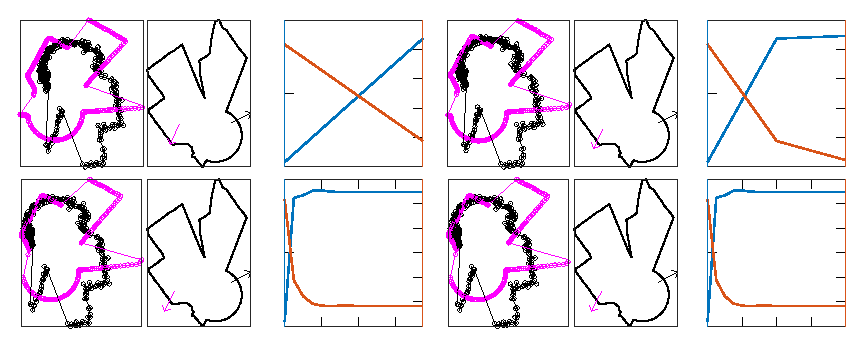
\includegraphics{./figures/parts/02/chapters/04/sections/04/sr5_sm0_fail_1}}%
    \gplfronttext
  \end{picture}%
\endgroup

    \end{subfigure}
  \vspace{0.5cm}
  \caption{\small Παράδειγμα εξέλιξης ανεπιτυχούς ευθυγράμμισης πραγματικής με
           εικονικές σαρώσεις μέσω της μεθόδου FSMSM. Η πραγματική στάση του
           αισθητήρα και η πραγματική σάρωση απεικονίζονται με μαύρο χρώμα, ενώ
           η εκτίμηση της στάσης και οι εικονικές σαρώσεις με ματζέντα. Τα
           διαγράμματα της τρίτης και έκτης στήλης απεικονίζουν με μπλε το
           ολικό σφάλμα εκτίμησης στάσης, και με κόκκινο την τιμή της μετρικής
           CAER}
  \label{fig:02_04_06:03}
\end{figure}

Οι κύριοι περιορισμοί της απόκρισης των προσθετικών μεθόδων ευθυγράμμισης
πραγματικών με εικονικές σαρώσεις αφορούν στα αμετάβλητα χαρακτηριστικά μεγέθη
του ίδιου του φυσικού αισθητήρα σαρώσεων, τα οποία είναι δυο. Το πρώτο είναι το
μέγεθος των διαταραχών που επιδρούν στις μετρήσεις του, την απόκριση επί του
οποίου εξετάσαμε για διάφορες τιμές στην ενότητα \ref{section:02_04_05}. Το
δεύτερο είναι το βεληνεκές του αισθητήρα, δηλαδή η μέγιστη απόσταση μέχρι την
οποία μπορεί να ανιχνεύσει την παρουσία αντικειμένων.

Στην άνω σειρά του σχήματος \ref{fig:02_04_06:04} εμφανίζονται με λευκό χρώμα
τέσσερα διαφορετικά περιβάλλοντα, μέσα στα οποία τοποθετείται ένας αισθητήρας
στις θέσεις που σημειώνονται με κουκκίδες βαθύ μπλε χρώματος. Οι θέσεις αυτές
είναι τα κέντρα των ομόκεντρων κύκλων που εμφανίζονται στην ίδια σειρά. Η
πειραματική διάταξη που ακολουθεί στοχεύει στην καταγραφή της απόκρισης
τεσσάρων κυρίων μεθόδων, ήτοι των PLICP, NDT, \texttt{x1}, και \texttt{uf}, σε
πειράματα όπου το βεληνεκές του αισθητήρα μεταβάλλεται έτσι ώστε οι μετρήσεις
του να περιλαμβάνουν όλα τα εμπόδια του περιβάλλοντος, μειούμενο μέχρι που να
μην περιλαμβάνουν κανένα. Το βεληνεκές του αισθητήρα είναι η ακτίνα των κύκλων
της πρώτης σειράς του σχήματος, και το χρώμα αυτών αναπαριστά το ποσοστό των
ακτίνων που φέρουν χωρική πληροφορία, βάσει της χρωματικής λωρίδας που
παρουσιάζεται στη δεύτερη σειρά. Στις δύο τελευταίες σειρές παρατίθενται οι
μέσοι όροι των ολικών σφαλμάτων εκτίμησης στάσης σε δέκα επαναλήψεις, για κάθε
μέθοδο και περιβάλλον, για $\sigma_R = \{0.01, 0.05\}$ m και $\sigma_{\bm{M}} =
0.0$ m. Η εκτίμηση θέσης και προσανατολισμού παράγεται τυχαία για κάθε πείραμα
μέσω διαταραχής των αντίστοιχων συνιστωσών της πραγματικής στάσης του αισθητήρα
με ποσότητες που εξάγονται από τις ομοιόμορφες κατανομές $U_{xy}(-0.20, +0.20)$
m και $U_{\theta}(-\pi/4,+\pi,4)$ rad.

\begin{figure}
  \begin{subfigure}{\linewidth}
    % GNUPLOT: LaTeX picture with Postscript
\begingroup
  \makeatletter
  \providecommand\color[2][]{%
    \GenericError{(gnuplot) \space\space\space\@spaces}{%
      Package color not loaded in conjunction with
      terminal option `colourtext'%
    }{See the gnuplot documentation for explanation.%
    }{Either use 'blacktext' in gnuplot or load the package
      color.sty in LaTeX.}%
    \renewcommand\color[2][]{}%
  }%
  \providecommand\includegraphics[2][]{%
    \GenericError{(gnuplot) \space\space\space\@spaces}{%
      Package graphicx or graphics not loaded%
    }{See the gnuplot documentation for explanation.%
    }{The gnuplot epslatex terminal needs graphicx.sty or graphics.sty.}%
    \renewcommand\includegraphics[2][]{}%
  }%
  \providecommand\rotatebox[2]{#2}%
  \@ifundefined{ifGPcolor}{%
    \newif\ifGPcolor
    \GPcolorfalse
  }{}%
  \@ifundefined{ifGPblacktext}{%
    \newif\ifGPblacktext
    \GPblacktexttrue
  }{}%
  % define a \g@addto@macro without @ in the name:
  \let\gplgaddtomacro\g@addto@macro
  % define empty templates for all commands taking text:
  \gdef\gplfronttext{}%
  \gdef\gplfronttext{}%
  \makeatother
  \ifGPblacktext
    % no textcolor at all
    \def\colorrgb#1{}%
    \def\colorgray#1{}%
  \else
    % gray or color?
    \ifGPcolor
      \def\colorrgb#1{\color[rgb]{#1}}%
      \def\colorgray#1{\color[gray]{#1}}%
      \expandafter\def\csname LTw\endcsname{\color{white}}%
      \expandafter\def\csname LTb\endcsname{\color{black}}%
      \expandafter\def\csname LTa\endcsname{\color{black}}%
      \expandafter\def\csname LT0\endcsname{\color[rgb]{1,0,0}}%
      \expandafter\def\csname LT1\endcsname{\color[rgb]{0,1,0}}%
      \expandafter\def\csname LT2\endcsname{\color[rgb]{0,0,1}}%
      \expandafter\def\csname LT3\endcsname{\color[rgb]{1,0,1}}%
      \expandafter\def\csname LT4\endcsname{\color[rgb]{0,1,1}}%
      \expandafter\def\csname LT5\endcsname{\color[rgb]{1,1,0}}%
      \expandafter\def\csname LT6\endcsname{\color[rgb]{0,0,0}}%
      \expandafter\def\csname LT7\endcsname{\color[rgb]{1,0.3,0}}%
      \expandafter\def\csname LT8\endcsname{\color[rgb]{0.5,0.5,0.5}}%
    \else
      % gray
      \def\colorrgb#1{\color{black}}%
      \def\colorgray#1{\color[gray]{#1}}%
      \expandafter\def\csname LTw\endcsname{\color{white}}%
      \expandafter\def\csname LTb\endcsname{\color{black}}%
      \expandafter\def\csname LTa\endcsname{\color{black}}%
      \expandafter\def\csname LT0\endcsname{\color{black}}%
      \expandafter\def\csname LT1\endcsname{\color{black}}%
      \expandafter\def\csname LT2\endcsname{\color{black}}%
      \expandafter\def\csname LT3\endcsname{\color{black}}%
      \expandafter\def\csname LT4\endcsname{\color{black}}%
      \expandafter\def\csname LT5\endcsname{\color{black}}%
      \expandafter\def\csname LT6\endcsname{\color{black}}%
      \expandafter\def\csname LT7\endcsname{\color{black}}%
      \expandafter\def\csname LT8\endcsname{\color{black}}%
    \fi
  \fi
    \setlength{\unitlength}{0.0300bp}%
    \ifx\gptboxheight\undefined%
      \newlength{\gptboxheight}%
      \newlength{\gptboxwidth}%
      \newsavebox{\gptboxtext}%
    \fi%
    \setlength{\fboxrule}{0.5pt}%
    \setlength{\fboxsep}{1pt}%
  \hspace{1cm}
\begin{picture}(8000.00,4000.00)%
    \gplgaddtomacro\gplfronttext{%
    }%
    \gplgaddtomacro\gplfronttext{%
    }%
    \gplgaddtomacro\gplfronttext{%
    }%
    \gplgaddtomacro\gplfronttext{%
    }%
    \gplgaddtomacro\gplfronttext{%
    }%
    \gplgaddtomacro\gplfronttext{%
    }%
    \gplgaddtomacro\gplfronttext{%
    }%
    \gplgaddtomacro\gplfronttext{%
    }%
    \gplgaddtomacro\gplfronttext{%
    }%
    \gplgaddtomacro\gplfronttext{%
      \colorrgb{0.00,0.00,0.00}%
      \put(3999,1499){\makebox(0,0){\strut{}\scriptsize Χρωματική αναπαράσταση ποσοστού ακτίνων εντός βεληνεκούς του αισθητήρα}}%
    }%
    \gplgaddtomacro\gplfronttext{%
    }%
    \gplgaddtomacro\gplfronttext{%
      \colorrgb{0.00,0.00,0.00}%
      \put(80,820){\makebox(0,0){\strut{}\scriptsize $0\%$}}%
      \colorrgb{1.00,1.00,1.00}%
      \put(1648,820){\makebox(0,0){\strut{}\scriptsize $20\%$}}%
      \colorrgb{1.00,1.00,1.00}%
      \put(3216,820){\makebox(0,0){\strut{}\scriptsize $40\%$}}%
      \colorrgb{1.00,1.00,1.00}%
      \put(4783,820){\makebox(0,0){\strut{}\scriptsize $60\%$}}%
      \colorrgb{1.00,1.00,1.00}%
      \put(6351,820){\makebox(0,0){\strut{}\scriptsize $80\%$}}%
      \colorrgb{1.00,1.00,1.00}%
      \put(7919,820){\makebox(0,0){\strut{}\scriptsize $100\%$}}%
    }%
    \put(0,0){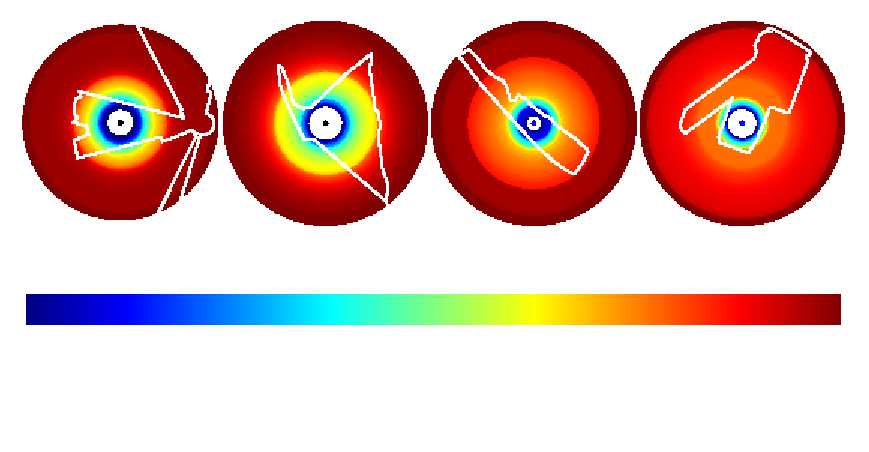
\includegraphics[scale=0.6]{./figures/slides/ch6/limitations/smsm_max_range_limitations_0}}%
    \gplfronttext
  \end{picture}%
\endgroup

  \end{subfigure}\\
  \begin{subfigure}{\linewidth}
    \definecolor{c1}{rgb}{0.290,0.435,0.890}
\definecolor{c2}{rgb}{0.710,0.733,0.890}
\definecolor{c7}{rgb}{0.902,0.686,0.725}
\definecolor{c8}{rgb}{0.827,0.247,0.416}

% GNUPLOT: LaTeX picture with Postscript
\begingroup
  \makeatletter
  \providecommand\color[2][]{%
    \GenericError{(gnuplot) \space\space\space\@spaces}{%
      Package color not loaded in conjunction with
      terminal option `colourtext'%
    }{See the gnuplot documentation for explanation.%
    }{Either use 'blacktext' in gnuplot or load the package
      color.sty in LaTeX.}%
    \renewcommand\color[2][]{}%
  }%
  \providecommand\includegraphics[2][]{%
    \GenericError{(gnuplot) \space\space\space\@spaces}{%
      Package graphicx or graphics not loaded%
    }{See the gnuplot documentation for explanation.%
    }{The gnuplot epslatex terminal needs graphicx.sty or graphics.sty.}%
    \renewcommand\includegraphics[2][]{}%
  }%
  \providecommand\rotatebox[2]{#2}%
  \@ifundefined{ifGPcolor}{%
    \newif\ifGPcolor
    \GPcolorfalse
  }{}%
  \@ifundefined{ifGPblacktext}{%
    \newif\ifGPblacktext
    \GPblacktexttrue
  }{}%
  % define a \g@addto@macro without @ in the name:
  \let\gplgaddtomacro\g@addto@macro
  % define empty templates for all commands taking text:
  \gdef\gplfronttext{}%
  \gdef\gplfronttext{}%
  \makeatother
  \ifGPblacktext
    % no textcolor at all
    \def\colorrgb#1{}%
    \def\colorgray#1{}%
  \else
    % gray or color?
    \ifGPcolor
      \def\colorrgb#1{\color[rgb]{#1}}%
      \def\colorgray#1{\color[gray]{#1}}%
      \expandafter\def\csname LTw\endcsname{\color{white}}%
      \expandafter\def\csname LTb\endcsname{\color{black}}%
      \expandafter\def\csname LTa\endcsname{\color{black}}%
      \expandafter\def\csname LT0\endcsname{\color[rgb]{1,0,0}}%
      \expandafter\def\csname LT1\endcsname{\color[rgb]{0,1,0}}%
      \expandafter\def\csname LT2\endcsname{\color[rgb]{0,0,1}}%
      \expandafter\def\csname LT3\endcsname{\color[rgb]{1,0,1}}%
      \expandafter\def\csname LT4\endcsname{\color[rgb]{0,1,1}}%
      \expandafter\def\csname LT5\endcsname{\color[rgb]{1,1,0}}%
      \expandafter\def\csname LT6\endcsname{\color[rgb]{0,0,0}}%
      \expandafter\def\csname LT7\endcsname{\color[rgb]{1,0.3,0}}%
      \expandafter\def\csname LT8\endcsname{\color[rgb]{0.5,0.5,0.5}}%
    \else
      % gray
      \def\colorrgb#1{\color{black}}%
      \def\colorgray#1{\color[gray]{#1}}%
      \expandafter\def\csname LTw\endcsname{\color{white}}%
      \expandafter\def\csname LTb\endcsname{\color{black}}%
      \expandafter\def\csname LTa\endcsname{\color{black}}%
      \expandafter\def\csname LT0\endcsname{\color{black}}%
      \expandafter\def\csname LT1\endcsname{\color{black}}%
      \expandafter\def\csname LT2\endcsname{\color{black}}%
      \expandafter\def\csname LT3\endcsname{\color{black}}%
      \expandafter\def\csname LT4\endcsname{\color{black}}%
      \expandafter\def\csname LT5\endcsname{\color{black}}%
      \expandafter\def\csname LT6\endcsname{\color{black}}%
      \expandafter\def\csname LT7\endcsname{\color{black}}%
      \expandafter\def\csname LT8\endcsname{\color{black}}%
    \fi
  \fi
    \setlength{\unitlength}{0.0500bp}%
    \ifx\gptboxheight\undefined%
      \newlength{\gptboxheight}%
      \newlength{\gptboxwidth}%
      \newsavebox{\gptboxtext}%
    \fi%
    \setlength{\fboxrule}{0.5pt}%
    \setlength{\fboxsep}{1pt}%
  \hspace{1cm}
\begin{picture}(8000.00,2400.00)%
    \gplgaddtomacro\gplfronttext{%
      \colorrgb{0.15,0.15,0.15}%
      \put(-52,1212){\makebox(0,0)[r]{\strut{}$0.0$}}%
      \colorrgb{0.15,0.15,0.15}%
      \put(-52,1445){\makebox(0,0)[r]{\strut{}$0.2$}}%
      \colorrgb{0.15,0.15,0.15}%
      \put(-52,1677){\makebox(0,0)[r]{\strut{}$0.4$}}%
      \colorrgb{0.15,0.15,0.15}%
      \put(-52,1910){\makebox(0,0)[r]{\strut{}$0.6$}}%
      \colorrgb{0.15,0.15,0.15}%
      \put(-52,2142){\makebox(0,0)[r]{\strut{}$0.8$}}%
      \colorrgb{0.15,0.15,0.15}%
      \put(-52,2375){\makebox(0,0)[r]{\strut{}$1.0$}}%
      \colorrgb{0.15,0.15,0.15}%
      \put(80,992){\makebox(0,0){\strut{}}}%
      \colorrgb{0.15,0.15,0.15}%
      \put(460,992){\makebox(0,0){\strut{}}}%
      \colorrgb{0.15,0.15,0.15}%
      \put(840,992){\makebox(0,0){\strut{}}}%
      \colorrgb{0.15,0.15,0.15}%
      \put(1219,992){\makebox(0,0){\strut{}}}%
      \colorrgb{0.15,0.15,0.15}%
      \put(1599,992){\makebox(0,0){\strut{}}}%
      \colorrgb{0.15,0.15,0.15}%
      \put(1979,992){\makebox(0,0){\strut{}}}%
      \put(1700,2600){\makebox(0,0){\strut{}{\color{c1}{\rule[0.6mm]{0.5cm}{0.5mm}}}\footnotesize PLICP}}
      \put(3100,2600){\makebox(0,0){\strut{}{\color{c2}{\rule[0.6mm]{0.5cm}{0.5mm}}}\footnotesize NDT}}
      \put(4400,2600){\makebox(0,0){\strut{}{\color{c7}{\rule[0.6mm]{0.5cm}{0.5mm}}}\footnotesize \texttt{x1}}}
      \put(5800,2600){\makebox(0,0){\strut{}{\color{c8}{\rule[0.6mm]{0.5cm}{0.5mm}}}\footnotesize \texttt{uf}}}
    }%
    \gplgaddtomacro\gplfronttext{%
      \colorrgb{0.15,0.15,0.15}%
      \put(-690,2000){\rotatebox{90}{\makebox(0,0){\strut{}$\sigma_R = 0.01$ m}}}%
      \put(-690,400){\rotatebox{90}{\makebox(0,0){\strut{}$\sigma_R = 0.05$ m}}}%
      \put(-1090,1200){\rotatebox{90}{\makebox(0,0){\strut{}Σφάλμα εκτίμησης στάσης}}}%
    }%
    \gplgaddtomacro\gplfronttext{%
      \colorrgb{0.15,0.15,0.15}%
      \put(-52,24){\makebox(0,0)[r]{\strut{}$0.0$}}%
      \colorrgb{0.15,0.15,0.15}%
      \put(-52,257){\makebox(0,0)[r]{\strut{}$0.2$}}%
      \colorrgb{0.15,0.15,0.15}%
      \put(-52,489){\makebox(0,0)[r]{\strut{}$0.4$}}%
      \colorrgb{0.15,0.15,0.15}%
      \put(-52,722){\makebox(0,0)[r]{\strut{}$0.6$}}%
      \colorrgb{0.15,0.15,0.15}%
      \put(-52,954){\makebox(0,0)[r]{\strut{}$0.8$}}%
      \colorrgb{0.15,0.15,0.15}%
      %\put(-52,1187){\makebox(0,0)[r]{\strut{}$1.0$}}%
      \colorrgb{0.15,0.15,0.15}%
      \put(80,-196){\makebox(0,0){\strut{}}}%
      \colorrgb{0.15,0.15,0.15}%
      \put(460,-196){\makebox(0,0){\strut{}\small $20\%$}}%
      \colorrgb{0.15,0.15,0.15}%
      \put(840,-196){\makebox(0,0){\strut{}}}%
      \colorrgb{0.15,0.15,0.15}%
      \put(1219,-196){\makebox(0,0){\strut{}\small $60\%$}}%
      \colorrgb{0.15,0.15,0.15}%
      \put(1599,-196){\makebox(0,0){\strut{}}}%
      \colorrgb{0.15,0.15,0.15}%
      \put(1979,-196){\makebox(0,0){\strut{}\small $100\%$}}%
    }%
    \gplgaddtomacro\gplfronttext{%
      \colorrgb{0.15,0.15,0.15}%
    }%
    \gplgaddtomacro\gplfronttext{%
      \colorrgb{0.15,0.15,0.15}%
      \put(1928,24){\makebox(0,0)[r]{\strut{}}}%
      \colorrgb{0.15,0.15,0.15}%
      \put(1928,257){\makebox(0,0)[r]{\strut{}}}%
      \colorrgb{0.15,0.15,0.15}%
      \put(1928,489){\makebox(0,0)[r]{\strut{}}}%
      \colorrgb{0.15,0.15,0.15}%
      \put(1928,722){\makebox(0,0)[r]{\strut{}}}%
      \colorrgb{0.15,0.15,0.15}%
      \put(1928,954){\makebox(0,0)[r]{\strut{}}}%
      \colorrgb{0.15,0.15,0.15}%
      \put(1928,1187){\makebox(0,0)[r]{\strut{}}}%
      \colorrgb{0.15,0.15,0.15}%
      \put(2060,-196){\makebox(0,0){\strut{}}}%
      \colorrgb{0.15,0.15,0.15}%
      \put(2440,-196){\makebox(0,0){\strut{}\small $20\%$}}%
      \colorrgb{0.15,0.15,0.15}%
      \put(2820,-196){\makebox(0,0){\strut{}}}%
      \colorrgb{0.15,0.15,0.15}%
      \put(3199,-196){\makebox(0,0){\strut{}\small $60\%$}}%
      \colorrgb{0.15,0.15,0.15}%
      \put(3579,-196){\makebox(0,0){\strut{}}}%
      \colorrgb{0.15,0.15,0.15}%
      \put(3959,-196){\makebox(0,0){\strut{}\small $100\%$}}%
    }%
    \gplgaddtomacro\gplfronttext{%
    }%
    \gplgaddtomacro\gplfronttext{%
      \colorrgb{0.15,0.15,0.15}%
      \put(3908,24){\makebox(0,0)[r]{\strut{}}}%
      \colorrgb{0.15,0.15,0.15}%
      \put(3908,257){\makebox(0,0)[r]{\strut{}}}%
      \colorrgb{0.15,0.15,0.15}%
      \put(3908,489){\makebox(0,0)[r]{\strut{}}}%
      \colorrgb{0.15,0.15,0.15}%
      \put(3908,722){\makebox(0,0)[r]{\strut{}}}%
      \colorrgb{0.15,0.15,0.15}%
      \put(3908,954){\makebox(0,0)[r]{\strut{}}}%
      \colorrgb{0.15,0.15,0.15}%
      \put(3908,1187){\makebox(0,0)[r]{\strut{}}}%
      \colorrgb{0.15,0.15,0.15}%
      \put(4040,-196){\makebox(0,0){\strut{}}}%
      \colorrgb{0.15,0.15,0.15}%
      \put(4420,-196){\makebox(0,0){\strut{}\small $20\%$}}%
      \colorrgb{0.15,0.15,0.15}%
      \put(4800,-196){\makebox(0,0){\strut{}}}%
      \colorrgb{0.15,0.15,0.15}%
      \put(5179,-196){\makebox(0,0){\strut{}\small $60\%$}}%
      \colorrgb{0.15,0.15,0.15}%
      \put(5559,-196){\makebox(0,0){\strut{}}}%
      \colorrgb{0.15,0.15,0.15}%
      \put(5939,-196){\makebox(0,0){\strut{}\small $100\%$}}%
    }%
    \gplgaddtomacro\gplfronttext{%
      \colorrgb{0.15,0.15,0.15}%
      \put(3999,-526){\makebox(0,0){\strut{}Ποσοστό ακτίνων εντός μέγιστου εύρους του αισθητήρα}}%

    }%
    \gplgaddtomacro\gplfronttext{%
      \colorrgb{0.15,0.15,0.15}%
      \put(5888,24){\makebox(0,0)[r]{\strut{}}}%
      \colorrgb{0.15,0.15,0.15}%
      \put(5888,257){\makebox(0,0)[r]{\strut{}}}%
      \colorrgb{0.15,0.15,0.15}%
      \put(5888,489){\makebox(0,0)[r]{\strut{}}}%
      \colorrgb{0.15,0.15,0.15}%
      \put(5888,722){\makebox(0,0)[r]{\strut{}}}%
      \colorrgb{0.15,0.15,0.15}%
      \put(5888,954){\makebox(0,0)[r]{\strut{}}}%
      \colorrgb{0.15,0.15,0.15}%
      \put(5888,1187){\makebox(0,0)[r]{\strut{}}}%
      \colorrgb{0.15,0.15,0.15}%
      \put(6020,-196){\makebox(0,0){\strut{}}}%
      \colorrgb{0.15,0.15,0.15}%
      \put(6400,-196){\makebox(0,0){\strut{}\small $20\%$}}%
      \colorrgb{0.15,0.15,0.15}%
      \put(6780,-196){\makebox(0,0){\strut{}}}%
      \colorrgb{0.15,0.15,0.15}%
      \put(7159,-196){\makebox(0,0){\strut{}\small $60\%$}}%
      \colorrgb{0.15,0.15,0.15}%
      \put(7539,-196){\makebox(0,0){\strut{}}}%
      \colorrgb{0.15,0.15,0.15}%
      \put(7919,-196){\makebox(0,0){\strut{}\small $100\%$}}%
    }%
    \gplgaddtomacro\gplfronttext{%
    }%
    \put(0,0){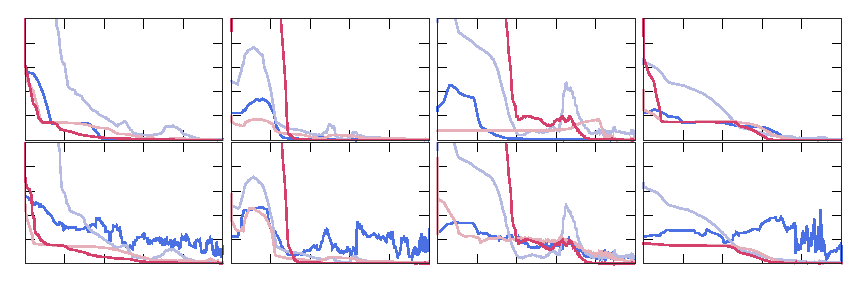
\includegraphics{./figures/parts/02/chapters/04/sections/06/smsm_max_range_limitations_1}}%
    \gplfronttext
  \end{picture}%
\endgroup

  \end{subfigure}
  \vspace{1cm}
  \caption{\small Πειράματα απόκρισης του σφάλματος εκτίμησης των PLICP, NDT,
           \texttt{x1} και \texttt{uf} σε συνθήκες μειούμενου
           βεληνεκούς-μέγιστου εύρους για δύο τιμές τυπικής απόκλισης των
           διαταραχών που επιδρούν στις μετρήσεις του φυσικού αισθητήρα όταν
           $\sigma_{\bm{M}} = 0.0$ m. Η απόκριση της μεθόδου \texttt{fm} είναι
           παρόμοια αυτής της μεθόδου \texttt{uf}}
  \label{fig:02_04_06:04}
\end{figure}

Στα διαγράμματα των τελευταίων δύο σειρών παρατηρούμε πως: (α) δεν υφίσταται
ομοιόμορφη απόκριση για οποιαδήποτε μέθοδο όσο αφορά σε κάθε περιβάλλον:
συνεπώς η απόκριση κάθε μεθόδου εξαρτάται και από τα χαρακτηριστικά του
εκάστοτε περιβάλλοντος, (β) η απόκριση της μεθόδου \texttt{uf} είναι παρόμοια
με την ονομαστική για ποσοστό αριθμού ακτίνων εντός του βεληνεκούς έως και
$80\%$ για κάθε περιβάλλον και επίπεδο διαταραχών υπό δοκιμή, (γ) η απόκριση
της μεθόδου \texttt{x1} εμφανίζει κατά μέσο όρο τα χαμηλότερα σφάλματα όταν
λαμβάνεται υπόψη ολόκληρο το εύρος των ποσοστών ακτίνων ($[0\%,100\%]$) εντός
του βεληνεκούς, (δ) το σφάλμα εκτίμησης της μεθόδου PLICP είναι το μέγιστο
ανάμεσα σε όλες τις υπό δοκιμή μεθόδους στο διάστημα $[50\%,100\%]$ των ακτίνων
όταν $\sigma_R = 0.05$ m για τρία από τα τέσσερα περιβάλλοντα, (ε) το σφάλμα
εκτίμησης της μεθόδου NDT αυξάνει με συνέπεια σε κάθε περιβάλλον και επίπεδο
διαταραχών υπό δοκιμή καθώς μειώνεται το ποσοστό των ακτίνων των οποίων οι
μετρήσεις βρίσκονται εντός του μέγιστου εύρους. Τούτων αναφερθέντων, δεν είναι
δυνατό να προκύψει κάποιο συμπέρασμα που για δεδομένο ποσοστό ακτίνων εντός
μέγιστου εύρους καθορίζει με συνέπεια την περισσότερο ακριβή μέθοδο
ευθυγράμμισης. Με βάση τα παραπάνω πειραματικά αποτελέσματα, η πιο συνετή
κίνηση όσο αφορά σε όλες τις προσθετικές μεθόδους ευθυγράμμισης είναι ο
πρότερος της ευθυγράμμισης υπολογισμός του ποσοστού των ακτίνων εντός του
βεληνεκούς του αισθητήρα, και η λήψη απόφασης ευθυγράμμισης ή μη, αναλόγως με
το είδος του περιβάλλοντος (δύσκολο έως αδύνατον) ή το είδος της μεθόδου (π.χ.
οι μέθοδοι \texttt{x1} και \texttt{uf} συμπεριφέρονται κατά προσέγγιση
ονομαστικά ως το $70\%$ των ακτίνων να βρίσκονται εντός του βεληνεκούς σε τρία
από τα τέσσερα υπό δοκιμή περιβάλλοντα, για κάθε επίπεδο διαταραχών των
μετρήσεων).
